\documentclass[a4paper,12pt,twoside]{memoir}

% Castellano
\usepackage[spanish,es-tabla]{babel}
\selectlanguage{spanish}
\usepackage[utf8]{inputenc}
\usepackage[T1]{fontenc}
\usepackage{lmodern} % scalable font
\usepackage{microtype}
\usepackage{placeins}
\usepackage{lscape}

\RequirePackage{booktabs}
\RequirePackage[table]{xcolor}
\RequirePackage{xtab}
\RequirePackage{multirow}

% Links
\PassOptionsToPackage{hyphens}{url}\usepackage[colorlinks]{hyperref}
\hypersetup{
	allcolors = {red}
}

% Ecuaciones
\usepackage{amsmath}

% Rutas de fichero / paquete
\newcommand{\ruta}[1]{{\sffamily #1}}

% Párrafos
\nonzeroparskip

% Huérfanas y viudas
\widowpenalty100000
\clubpenalty100000

% Evitar solapes en el header
\nouppercaseheads

% Imagenes
\usepackage{graphicx}
\newcommand{\imagen}[2]{
	\begin{figure}[!h]
		\centering
		\includegraphics[width=0.9\textwidth]{#1}
		\caption{#2}\label{fig:#1}
	\end{figure}
	\FloatBarrier
}

\newcommand{\imagenflotante}[2]{
	\begin{figure}%[!h]
		\centering
		\includegraphics[width=0.9\textwidth]{#1}
		\caption{#2}\label{fig:#1}
	\end{figure}
}



% El comando \figura nos permite insertar figuras comodamente, y utilizando
% siempre el mismo formato. Los parametros son:
% 1 -> Porcentaje del ancho de página que ocupará la figura (de 0 a 1)
% 2 --> Fichero de la imagen
% 3 --> Texto a pie de imagen
% 4 --> Etiqueta (label) para referencias
% 5 --> Opciones que queramos pasarle al \includegraphics
% 6 --> Opciones de posicionamiento a pasarle a \begin{figure}
\newcommand{\figuraConPosicion}[6]{%
  \setlength{\anchoFloat}{#1\textwidth}%
  \addtolength{\anchoFloat}{-4\fboxsep}%
  \setlength{\anchoFigura}{\anchoFloat}%
  \begin{figure}[#6]
    \begin{center}%
      \Ovalbox{%
        \begin{minipage}{\anchoFloat}%
          \begin{center}%
            \includegraphics[width=\anchoFigura,#5]{#2}%
            \caption{#3}%
            \label{#4}%
          \end{center}%
        \end{minipage}
      }%
    \end{center}%
  \end{figure}%
}

%
% Comando para incluir imágenes en formato apaisado (sin marco).
\newcommand{\figuraApaisadaSinMarco}[5]{%
  \begin{figure}%
    \begin{center}%
    \includegraphics[angle=90,height=#1\textheight,#5]{#2}%
    \caption{#3}%
    \label{#4}%
    \end{center}%
  \end{figure}%
}
% Para las tablas
\newcommand{\otoprule}{\midrule [\heavyrulewidth]}
%
% Nuevo comando para tablas pequeñas (menos de una página).
\newcommand{\tablaSmall}[5]{%
 \begin{table}
  \begin{center}
   \rowcolors {2}{gray!35}{}
   \begin{tabular}{#2}
    \toprule
    #4
    \otoprule
    #5
    \bottomrule
   \end{tabular}
   \caption{#1}
   \label{tabla:#3}
  \end{center}
 \end{table}
}

%
%Para el float H de tablaSmallSinColores
\usepackage{float}

%
% Nuevo comando para tablas pequeñas (menos de una página).
\newcommand{\tablaSmallSinColores}[5]{%
 \begin{table}[H]
  \begin{center}
   \begin{tabular}{#2}
    \toprule
    #4
    \otoprule
    #5
    \bottomrule
   \end{tabular}
   \caption{#1}
   \label{tabla:#3}
  \end{center}
 \end{table}
}

\newcommand{\tablaApaisadaSmall}[5]{%
\begin{landscape}
  \begin{table}
   \begin{center}
    \rowcolors {2}{gray!35}{}
    \begin{tabular}{#2}
     \toprule
     #4
     \otoprule
     #5
     \bottomrule
    \end{tabular}
    \caption{#1}
    \label{tabla:#3}
   \end{center}
  \end{table}
\end{landscape}
}

%
% Nuevo comando para tablas grandes con cabecera y filas alternas coloreadas en gris.
\newcommand{\tabla}[6]{%
  \begin{center}
    \tablefirsthead{
      \toprule
      #5
      \otoprule
    }
    \tablehead{
      \multicolumn{#3}{l}{\small\sl continúa desde la página anterior}\\
      \toprule
      #5
      \otoprule
    }
    \tabletail{
      \hline
      \multicolumn{#3}{r}{\small\sl continúa en la página siguiente}\\
    }
    \tablelasttail{
      \hline
    }
    \bottomcaption{#1}
    \rowcolors {2}{gray!35}{}
    \begin{xtabular}{#2}
      #6
      \bottomrule
    \end{xtabular}
    \label{tabla:#4}
  \end{center}
}

%
% Nuevo comando para tablas grandes con cabecera.
\newcommand{\tablaSinColores}[6]{%
  \begin{center}
    \tablefirsthead{
      \toprule
      #5
      \otoprule
    }
    \tablehead{
      \multicolumn{#3}{l}{\small\sl continúa desde la página anterior}\\
      \toprule
      #5
      \otoprule
    }
    \tabletail{
      \hline
      \multicolumn{#3}{r}{\small\sl continúa en la página siguiente}\\
    }
    \tablelasttail{
      \hline
    }
    \bottomcaption{#1}
    \begin{xtabular}{#2}
      #6
      \bottomrule
    \end{xtabular}
    \label{tabla:#4}
  \end{center}
}

%
% Nuevo comando para tablas grandes sin cabecera.
\newcommand{\tablaSinCabecera}[5]{%
  \begin{center}
    \tablefirsthead{
      \toprule
    }
    \tablehead{
      \multicolumn{#3}{l}{\small\sl continúa desde la página anterior}\\
      \hline
    }
    \tabletail{
      \hline
      \multicolumn{#3}{r}{\small\sl continúa en la página siguiente}\\
    }
    \tablelasttail{
      \hline
    }
    \bottomcaption{#1}
  \begin{xtabular}{#2}
    #5
   \bottomrule
  \end{xtabular}
  \label{tabla:#4}
  \end{center}
}



\definecolor{cgoLight}{HTML}{EEEEEE}
\definecolor{cgoExtralight}{HTML}{FFFFFF}

%
% Nuevo comando para tablas grandes sin cabecera.
\newcommand{\tablaSinCabeceraConBandas}[5]{%
  \begin{center}
    \tablefirsthead{
      \toprule
    }
    \tablehead{
      \multicolumn{#3}{l}{\small\sl continúa desde la página anterior}\\
      \hline
    }
    \tabletail{
      \hline
      \multicolumn{#3}{r}{\small\sl continúa en la página siguiente}\\
    }
    \tablelasttail{
      \hline
    }
    \bottomcaption{#1}
    \rowcolors[]{1}{cgoExtralight}{cgoLight}

  \begin{xtabular}{#2}
    #5
   \bottomrule
  \end{xtabular}
  \label{tabla:#4}
  \end{center}
}




\graphicspath{ {./img/} }

% Capítulos
\chapterstyle{bianchi}
\newcommand{\capitulo}[2]{
	\setcounter{chapter}{#1}
	\setcounter{section}{0}
	\setcounter{figure}{0}
	\setcounter{table}{0}
	\chapter*{#2}
	\addcontentsline{toc}{chapter}{#2}
	\markboth{#2}{#2}
}

% Apéndices
\renewcommand{\appendixname}{Apéndice}
\renewcommand*\cftappendixname{\appendixname}

\newcommand{\apendice}[1]{
	%\renewcommand{\thechapter}{A}
	\chapter{#1}
}

\renewcommand*\cftappendixname{\appendixname\ }

% Formato de portada
\makeatletter
\usepackage{xcolor}
\newcommand{\tutor}[1]{\def\@tutor{#1}}
\newcommand{\course}[1]{\def\@course{#1}}
\definecolor{cpardoBox}{HTML}{E6E6FF}
\def\maketitle{
  \null
  \thispagestyle{empty}
  % Cabecera ----------------
\noindent
\includegraphics[width=\textwidth]{cabecera}\vspace{1cm}%
  \vfill
  % Título proyecto y escudo informática ----------------
  \colorbox{cpardoBox}{%
    \begin{minipage}{.8\textwidth}
      \vspace{.5cm}\Large
      \begin{center}
      \textbf{TFG del Grado en Ingeniería Informática}\vspace{.6cm}\\
      \textbf{\LARGE\@title{}}
      \end{center}
      \vspace{.2cm}
    \end{minipage}

  }%
  \hfill\begin{minipage}{.20\textwidth}
    
\includegraphics[width=\textwidth]{escudoInfor}
  \end{minipage}
  \vfill
  % Datos de alumno, curso y tutores ------------------
  \begin{center}%
  {%
    \noindent\LARGE
    Presentado por \@author{}\\ 
    en Universidad de Burgos --- \@date{}\\
    Tutores: \@tutor{}\\
  }%
  \end{center}%
  \null
  \cleardoublepage
  }
\makeatother


% Datos de portada
\title{Plataforma de Corrección Automática de Ejercicios en Python}
\author{Alberto Porres Fernández}
\tutor{Bruno Baruque Zanón\\ y Roberto Carlos Casado Vara}
\date{7 de julio de 2022}

\begin{document}

\maketitle



\cleardoublepage



%%%%%%%%%%%%%%%%%%%%%%%%%%%%%%%%%%%%%%%%%%%%%%%%%%%%%%%%%%%%%%%%%%%%%%%%%%%%%%%%%%%%%%%%



\frontmatter


\clearpage

% Indices
\tableofcontents

\clearpage

\listoffigures

\clearpage

\listoftables

\clearpage

\mainmatter

\appendix

\apendice{Plan de Proyecto Software}

\section{Introducción}
En este primer apéndice se van a exponer los distintos \textit{sprints} que se han realizado durante el desarrollo del proyecto junto con un estudio de la viabilidad de este dividido en dos apartados: viabilidad económica y viabilidad legal.
\section{Planificación temporal}
Como ya se ha mencionado anteriormente, al desarrollo de este proyecto le ha sido aplicada una metodología \textit{agile}. Para posibilitar la adaptación de esta metodología a un proyecto supervisado, realizado por una sola persona, se han seguido las siguientes indicaciones:
\begin{itemize}
\item El desarollo ha sido dividido en \textit{sprints} de dos semanas de duración.
\item Al inicio de cada sprint eran definidas las tareas a realizar dentro de este, añadiéndose nuevas durante el desarrollo del sprint en caso de finalización de las incialmente definidas o por necesidades surgidas en el desarrollo de otras tareas y pasadas al siguiente sprint en caso de la no finalización de estas.
\item Se organizaban reuniones de supervisión alrededor de la fecha de finalización de cada sprint para comprobar el estado de cada tarea y su correcta superación.
\item A cada tarea le era asignado un coste estimado en formato de tiempo (horas) que el programador decidía de manera personal al definirse cada tarea.
\item Al darse por concluida una tarea se especificaba el coste real que esta había supuesto.
\end{itemize}
La gestión de tareas y la estimación de sus costes se ha realizado mediante la herramienta \textit{ZenHub}\cite{tool:ZenHub} mencionada en el apartado de Técnicas y Herramientas de la memoria.

A continuación se describirán los \textit{sprints} por los que este proyecto ha pasado:

\subsection{Sprint 1 (22/03/22 - 05/04/22)}
Este sprint consistió en una primera toma de contacto con las herramientas de autograding en Python\cite{tool:Python}. Momento del proyecto orientado hacia la investigación y aprendizaje ya que se trataba del inicio de este. Adicionalmente, se incluyó en este sprint la búsqueda de un curso\cite{PythonParaTodos} introductorio a Python sobre el que basar el que posteriormente sería nuestro curso y la redacción del apartado de objetivos de la memoria:

\begin{table}[h]
\begin{center}
\begin{tabular}{| l | c | c |}
\textbf{Tarea}                   & \textbf{Est} & \textbf{Real} \\ \hline
Búsqueda de atuograders, comparativa y elección & 1 & 6 \\
Búsqueda del curso de Python & 1 & 1 \\
Instalación y pruebas documentadas del autograder &  & \\
seleccionado & 8 & 8 \\
Completar apartado Objetivos en la memoria & 8 & - \\ \hline
\end{tabular}
\caption{Tareas sprint 1}
\label{tab:sprint}
\end{center}
\end{table}

\subsection{Sprint 2 (05/04/22 - 19/04/22)}
Al no poder ser realizada / finalizada la redacción del apartado de objetivos en el sprint inicial, esta tarea fue delegada a este sprint número 2 la cual pasó a ser la primera tarea de este. 

Una vez realizada la primera toma de contacto con la herramienta de autograding seleccionada \textit{Nbgrader}\cite{tool:Nbgrader}, se definieron para este sprint las tareas de adición de la documentación sobre la instalación y prueba de esta al Apéndice de Diseño, junto con la realización de una investigación sobre su funcionamiento interno. Además se añadió la tarea de creación de nuestro curso introductorio a Python junto con sus pruebas autocorregibles en un futuro mediante la herramienta Nbgrader. 

\begin{table}[h]
\begin{center}
\begin{tabular}{| l | c | c |}
\textbf{Tarea}                   & \textbf{Est} & \textbf{Real} \\ \hline
Completar apartado Objetivos en la memoria & 8 & 3 \\
Añadir la documentación de prueba e instalación de Nbgrader & &\\
a los anexos & 2 & 2 \\
Realizar investigación del funcionamiento interno de Nbgrader & 13 & 12 \\
Creación del curso de Python & 13 & 14 \\ \hline
\end{tabular}
\caption{Tareas sprint 3}
\label{tab:sprint}
\end{center}
\end{table}

\subsection{Sprint 3 (19/04/22 - 03/05/22)}
Finalizadas de forma exitosa todas las tareas del sprint 2, comenzaba así el sprint número 3 para el que fue definida la tarea de redacción de una explicación del funcionamiento de Nbgrader basada en la información obtenida en la tarea de investigación del sprint anterior.

Adicionalmente y como paso previo al inicio del desarrollo de la plataforma, era necesaria la prueba de ejecución y acceso a Jupyter Notebooks de forma remota en un contenedor Docker\cite{tool:Docker}, tarea que fue incluida en este sprint.

\begin{table}[h]
\begin{center}
\begin{tabular}{| l | c | c |}
\textbf{Tarea}                   & \textbf{Est} & \textbf{Real} \\ \hline
Jupyter Notebooks en Docker & 13 & 13 \\
Redactar explicación sobre el funcionamiento de Nbgrader & 5 & - \\ \hline
\end{tabular}
\caption{Tareas sprint 3}
\label{tab:sprint}
\end{center}
\end{table}



\subsection{Sprint 4 (03/05/22 - 17/05/22)}
Debido a que la completitud de la tarea de redacción de explicación sobre el funcionamiento de Nbgrader no había sido posible en el sprint número 3, esta tarea fue delegada a este cuarto sprint, tarea que fue acompañada con el comienzo del desarrollo de la plataforma web la cual contenía: la creación del login\cite{tool:FlaskLogin} inicial con \textit{Flask}, una prueba de acceso a Jupyter Notebooks\cite{tool:JupyterNotebooks} ejecutado remotamente en un contenedor docker junto con el proyecto Flask, el desarrollo del diagrama de casos de uso inicialmente pensado para la plataforma y el inicio de la implementación de las vistas y funcionalidades para los alumnos.



\begin{table}[h]
\begin{center}
\begin{tabular}{| l | c | c |}
\textbf{Tarea}                   & \textbf{Est} & \textbf{Real} \\ \hline
Redactar explicación sobre el funcionamiento de Nbgrader & 5 & 6 \\
Creación de nuestro primer login con Flask & 5 & 6 \\
Acceso a Jupyter Notebooks ejecutado remotamente & & \\
desde una aplicación Flask & 5 & 5 \\
Creación del diagrama de casos de uso & 2 & 2 \\
Desarrollo de las vistas de la aplicación para los alumnos & 21 & - \\\hline
\end{tabular}
\caption{Tareas sprint 4}
\label{tab:sprint}
\end{center}
\end{table}


\subsection{Sprint 5 (17/05/22 - 31/05/22)}
El sprint 5 fue dedicado en su totalidad al desarrollo de las vistas y funcionalidades de la aplicación para los alumnos, tarea de la que surgieron otras sub-tareas en su desarrollo que consistían en: prueba y adaptación de la API de Nbgrader\cite{tool:NbgraderAPI} a las funcionalidades implementándose en el momento y construcción de las tablas de la base de datos\cite{tool:SQLAlchemy}\cite{tool:SQLite} e inicialización de esta.



\begin{table}[h]
\begin{center}
\begin{tabular}{| l | c | c |}
\textbf{Tarea}                   & \textbf{Est} & \textbf{Real} \\ \hline
Desarrollo de las vistas de la aplicación para los alumnos & 21 & 24 \\
  (sub-tarea) Prueba y adaptación API de Nbgrader & 2 & 2 \\
  (sub-tarea) Inicialización de la base de datos & 5 & 5 \\\hline
\end{tabular}
\caption{Tareas sprint 5}
\label{tab:sprint}
\end{center}
\end{table}

\subsection{Sprint 6 (31/05/22 - 14/06/22)}
Tras la finalización del desarrollo de las funcionalidades para los estudiantes, se definía en el sprint 6 la tarea de desarrollo de las vistas y funcionalidades de la aplicación para el profesor, de la cual se generaron las sub-tareas de: desarrollo de funcionalidad de gestión completa de alumnos, funcionalidad de visualización de calificaciones por parte del profesor, funcionalidad de gestión completa de cursos.

Adicionalmente, en este sprint también se definieron otras tareas de menor carga de trabajo como el desarrollo del diagrama de clases de la base de datos y el diseño de un estado inicial para la plataforma, con el curso de Python, alumnos y entregas ya realizadas, estado incial que sería incluido en la plataforma posteriormente tras el despliegue vacío de esta.

También fue definida las tareas de creación del landing y adición de estilos y las vistas de la plataforma, siendo esta última únicamente iniciada durante este sprint.


\begin{table}[h]
\begin{center}
\begin{tabular}{| l | c | c |}
\textbf{Tarea}                   & \textbf{Est} & \textbf{Real} \\ \hline
Desarrollo de las vistas y funcionalidades de la aplicación & &\\
para el profesor & 21 & 30 \\
 (sub-tarea) Gestión completa de alumnos & 5 & 5 \\
 (sub-tarea) Gestión de calificaciones & 2 & 2 \\
 (sub-tarea) Gestión completa de cursos & 13 & 13 \\
Desarrollo diagrama de clases de la base de datos & 2 & 2 \\
Establecer el contenido incial que tendrá la plataforma & 2 & 2 \\
Creación del landing de la plataforma & 2 & 2\\
Dar estilos a toda la plataforma con Bootstrap y landing con CSS
 & 21 & - \\ \hline
\end{tabular}
\caption{Tareas sprint 6}
\label{tab:sprint}
\end{center}
\end{table}


\subsection{Sprint 7 (14/06/22 - 28/06/22)}
Añadidas todas las funcionalidades incialmente pensadas para la plataforma, el sprint 7 iniciaba con el final de la tarea de adición de estilos y creación de landing con Bootstrap\cite{tool:Bootstrap} y CSS\cite{tool:CSS} y en este eran definidas las tareas de: adición de nuevas funcionalidades (obtención de feedback, eliminación de entregas, descarga de tareas enviadas, eliminación de cursos y secciones), despliegue de la app en una instancia EC2 de AWS\cite{tool:AWS} y completitud de apartados de la memoria del proyecto.

\begin{table}[H]
\begin{center}
\begin{tabular}{| l | c | c |}
\textbf{Tarea}                   & \textbf{Est} & \textbf{Real} \\ \hline
Dar estilos a toda la plataforma con bootstrap y landing con CSS
 & 21 & 21 \\
Añadir funcionalidad de obtención de feedback & 3 & 1 \\
Añadir funcionalidad de eliminación de entregas & 2 & 2 \\
Añadir funcionalidad de eliminación de cursos y secciones & 3 & 3 \\
Añadir funcionalidad de descarga de envíos & 2 & 2 \\
Completar apartado Técnicas y Herramientas en la memoria & 5 & 4 \\ 
Completar apartado Aspectos Relevantes en la memoria & 5 & 4 \\ 
Completar apartados de Introducción, Conceptos Teóricos, & &\\
Trabajos Relacionados y Conclusiones & 8 & 8 \\ \hline
\end{tabular}
\caption{Tareas sprint 7}
\label{tab:sprint}
\end{center}
\end{table}


\subsection{Sprint 8 (28/06/22 - 07/07/22)}
El sprint número 8 da como concluido el proyecto, incluyéndose en este tareas dedicadas al desarrollo de los anexos y la adición de los contenidos definidos previamente a la plataforma ya desplegada.


\begin{table}[H]
\begin{center}
\begin{tabular}{| l | c | c |}
\textbf{Tarea}                   & \textbf{Est} & \textbf{Real} \\ \hline
Completar anexo Plan de Proyecto Software & 3 & 3 \\
Completar anexo Especificación de Requisitos & 3 & 3 \\
Completar anexo Especificación de Diseño & 3 & 3 \\ 
Completar anexo Documentación del Programador & 5 & 5 \\
Completar anexo Documentación del Usuario & 8 & 8 \\ 
Adición de contenidos a la plataforma desplegada & 2 & 2\\\hline
\end{tabular}
\caption{Tareas sprint 8}
\label{tab:sprint}
\end{center}
\end{table}



\section{Estudio de viabilidad}

\subsection{Viabilidad económica}
Analizaremos los costes en que habría incurrido el desarrollo de este proyecto de haberse
llevado a cabo en un ámbito empresarial o si se hubiese encargado a una entidad externa.

La estructura de costes la desglosaremos en los apartados coste de personal , costes de
software y costes del hardware y costes de estructura.

En cuanto a los ingresos o beneficios por la aplicación desarrollada no se realizada nigún
análisis. La razón es que no está previsto un uso comercial del producto generado, sino que
sería una herramienta utilizable dentro de un marco más general de formación en el que puede
haber otras herramientas empleadas. En dicho marco la mayor parte del valor añadido y de la
que se han de considerar los ingresos es la actividad realizada por los profesores: desarrollo del material de cursos, evaluaciones, tutorías y comunicaciones con alumnos, gestión de alumnos, etc.

\subsubsection{Costes de personal}
Para llevar a término el proyecto se ha requerido de un desarrollador durante un periodo de
cuatro meses. Si bien el tiempo de desarrollo es inferior al señalado hay que incluir también el dedicado al análisis de herramientas y estudio de soluciones. El coste de personal se desglosa en la siguiente tabla:

\begin{table}[H]
\begin{center}
\begin{tabular}{| l | c |} \hline
\textbf{Concepto}   & \textbf{Coste mensual (€)}  \\ \hline
Salario bruto  & 1500,00 \\
Seguridad Social (29,90 \%)  & 449,50\\
Coste para el empleador  & 1949,50 \\ \hline
Total Coste de personal (4 meses)  & 7794,00 €\\ \hline
\end{tabular}
\caption{Costes de personal}
\end{center}
\end{table}


El salario bruto incluye todo el montante del salario del trabajador por este concepto, es decir, integra la parte de prorrata de pagas extra. Para hallar el sueldo mensual neto del trabajador se debe descontar la prorrata de pagas extra (1 / 6 del bruto mensual) y la parte de Seguridad Social a cuenta del trabajador, que es el 6,35 \% del bruto mensual (incluyen los apartados contingencias comunes, desempleo y formación profesional).

El apartado de Seguridad incluye la parte a cuenta de la empresa por contingencias comunes
(23,60 \%), desempleo (5,50 \%), FOGASA (0,20 \%) y formación profesional (0,60 \%), según las tablas de la Seguridad Social para 2022.

\subsubsection{Costes de hardware}
Para este apartado se considera que se ha utilizado un ordenador portátil y ha sido necesario un teléfono móvil a cuenta de la empresa y disposición del trabajador. La amortización se consideran 4 años para ambos, con valor residual cero a final de dicho periodo.


\begin{table}[H]
\begin{center}
\begin{tabular}{| l | c | c |} \hline
\textbf{Equipo}   & \textbf{Coste (€)} & \textbf{Coste amortización 4 meses (€)}  \\ \hline
Ordenador portátil & 900,00 & 75,00 \\
Teléfono móvil & 264,00 & 22,00\\  \hline 
Total & 1164,00 & 97,00\\ \hline

\end{tabular}
\caption{Costes de hardware}
\end{center}
\end{table}



\subsubsection{Costes de software}
En este apartado se considera el coste de aquellas licencias de software necesarias y que no sean gratuitas.

En nuestro caso, esto afecta a las licencias de sistema operativo de los equipos hardware
empleado. No obstante, en el apartado relativo al hardware el coste total del equipo ya incluye el de la licencia de sistema operativo que llevan instalado de origen. El coste de amortización de dicho software se considera igual que el del equipo, pues no se prevé renovación del sistema operativo del equipo durante su vida útil. Es decir, que el coste del software de está ya incluido en el coste del apartado anterior.

\subsubsection{Costes de estructura}
En este apartado se incluyen costes aplicables al entorno de trabajo por parte de la empresa y servicios para que la funcionalidad del pruesto de trabajo sea operativa.

Se considera que el trabajo se ha realizado en modo teletrabajo, por lo que no se precisa una oficina operativa para el trabajador o un puesto destinado para él en una oficina. Esto resulta en que no se contemplan los costes asociados de alquiler de oficina, instalaciones, suministros eléctricos, limpieza, etc. No obstante, el trabajador necesita que se ponga a su disposición una conexión a Internet. Además necesita una compensación por el gasto de consumo eléctrico que requiera durante su trabajo, pues de otro modo correría por su cuenta.

\begin{table}[H]
\begin{center}
\begin{tabular}{| l | c |} \hline
\textbf{Concepto}   & \textbf{Coste mensual (€)}  \\ \hline
Conexión a internet & 30\\
Compensación por gasto eléctrico & 10\\
Coste por mes & 40 \\ \hline
Total Coste de estructura (4 meses)  & 160 €\\ \hline
\end{tabular}
\caption{Costes de estructura}
\end{center}
\end{table}

\subsubsection{Costes totales}

\begin{table}[H]
\begin{center}
\begin{tabular}{| l | c |} \hline
\textbf{Capítulo}   & \textbf{Coste (€)}  \\ \hline
Personal & 7.794,00\\
Hardware/Software & 97,00\\
Estructura &  160,00 \\ \hline
Total  & 8.051,00 €\\ \hline
\end{tabular}
\caption{Costes totales}
\end{center}
\end{table}



\subsection{Viabilidad legal}
En este apartado se consideran las licencias de software de terceras partes empleado en este proyecto.  Se analiza su repercusión o influencia en la viabilidad legal dado que su uso puede aparejar limitaciones o restricciones legales.

La siguiente tabla contiene las licencias de las diferentes herramientas empleadas:

\begin{table}[H]
\begin{center}
\begin{tabular}{| l | c |} \hline
\textbf{Herramienta}   & \textbf{Licencia}  \\ \hline
Python	&		PSF \\
Flask	&		BSD 3-clause \\
Flask-Login	&	BSD 3-clause\\ 
Flask-SQLAlchemy &	BSD 3-clause\\
SQLite	&		No se requiere\\
WTForms	&	BSD 3-clause\\
Nbgrader	&	BSD 3-clause\\
JavaScript	&	GNU-GPL-3.0\\
Bootstrap &		MIT License\\
Jupyter Notebook &	BSD 3-clause\\
Docker	&		Apache License 2.0\\\hline
\end{tabular}
\caption{Tabla de licencias}
\end{center}
\end{table}


Se describen a continuación estas licencias:

\begin{itemize}
\item \textbf{BSD}: Las licencias BSD son una familia de licencias de software libre permisivas , que imponen restricciones mínimas sobre el uso y distribución del software cubierto. Actualmente son de uso generalizado licencias BSD modificadas respecto a la licencia BSD que se estableció originalmente para la versión BSD de unix. La licencia BSD simplemente requiere que todo el código conserve el aviso de licencia BSD si se redistribuye en formato de código fuente, o que reproduzca el aviso si se redistribuye en formato binario. La licencia BSD 3-clause contiene un descargo de responsabilidad en la documentación y materiales proporcionados con la distribución. Además no pueden utilizarse sin permiso con fines de respaldo o promoción los nombres del titular de los derechos de autor ni de sus colaboradores.

\item \textbf{GNU-GPLv3}:  Esta licencia permite el uso comercial del software, su distribución, modificación y uso privado. Quien haga alguno de los usos anteriores está obligado a licenciar como código libre cualquier modificación del código o herramientas incorporadas con esta licencia.

\item \textbf{Apache 2.0}: Esta licencia tiene propiedades iguales que la licencia GPLv3. No obstante, no obliga a que los nuevos desarrollos con dependencias con Apache 2.0 se licencien como código libre.

\item \textbf{MIT}: La licencia MIT permite uso comercial del software licenciado, su modificación, su libre distribución y el uso privado. No presenta garantías ni responsabilidad. La única condición que impone es hacer referencia a tal licencia. No obliga a mantener la licencia, ni limita la distribución del software que use productos bajo esta licencia. Esto implica que la licencia final puede ser cualquiera.

\item \textbf{PSF}: Es una licencia de software libre, que al modo de BSD, es permisiva. Cumple con los requisitos OSI de licencia de software libre y es compatible con la licencia GPL. Al modo de las licencias BSD, permite modificaciones del código fuente y la creación de trabajos derivados, y no obliga a que tales modificaciones ni trabajos derivados tengan que ser a su vez de código abierto.
\end{itemize}

De todas las licencias descritas con anterioridad, la más restrictiva es la licencia GPLv3 la cual
ha sido aplicada a nuestra aplicación una vez desarrollada, permitiendo tanto su uso comercial como privado.


\apendice{Especificación de Requisitos}

\section{Introducción}
En este anexo se van a exponer las especificaciones de requisitos que definen el funcionamiento de la plataforma, comenzando por un repaso de objetivos de esta, exponiéndose los requisitos funcionales y no funcionales derivados de estos y finalizando con la exposición de los casos de uso resultantes de su desarrollo.

\section{Objetivos generales}
Como había sido mencionado previamente en la memoria, el objetivo principal de este proyecto consistía en el desarrollo de una plataforma web orientada a la enseñanza online la cual permita corregir de forma automática ejercicios en Python. Para ello, la plataforma debía basarse en la inclusión de cursos de carácter didáctico por parte de los profesores en los que se encontrarían las tareas y los contenidos teóricos de estos.

\newpage

\section{Catálogo de requisitos}
En esta sección son enumerados y descritos los requisitos funcionales y no funcionales derivados del objetivo descrito con anterioridad.

\subsection{Requisitos funcionales de un usuario sin autenticar:}
\begin{itemize}
\tightlist
\item
  \textbf{RF-1 Inicio de sesión:} Un usuario inicia sesión en la plataforma y es identificado
  como profesor o estudiante y llevado a la página principal correspondiente.
  
\end{itemize}

\subsection{Requisitos funcionales orientados al profesor:}
\begin{itemize}
\tightlist

\item
  \textbf{RF-2 Gestionar cursos:} Un profesor debe poder realizar la gestión de sus cursos.
  
  \begin{itemize}
  \tightlist
  \item
    \textbf{RF-2.1 Gestionar contenidos de un curso:} Un profesor debe poder gestionar los contenidos de cada curso.

    \begin{itemize}
    \tightlist
    \item
      \textbf{RF-2.1.1: Descargar contenidos y tareas:} Un profesor debe poder descargar los contenidos teóricos y tareas tanto en versión alumno como versión profesor de las secciones contenidas en el curso.
      
    \item  
      \textbf{RF-2.1.2: Gestionar secciones no publicadas:} Un profesor debe poder acceder a la gestión de las secciones no publicadas de ese curso.
      
      \begin{itemize}
      \tightlist
      \item
        \textbf{RF-2.1.2.1: Crear sección no publicada:} Un profesor debe poder crear nuevas secciones no publicadas para un curso.
        
      \item
        \textbf{RF-2.1.2.2: Editar tarea:} Un profesor debe poder editar las tareas de las secciones no publicada desde la propia plataforma.
        
      \item
        \textbf{RF-2.1.2.3: Descargar estado de la tarea:} Un profesor debe poder descargarse el estado actual en el que se encuentran las tareas de las seccies no publicadas.
        
      \item
        \textbf{RF-2.1.2.4: Eliminar sección no publicada:} Un profesor debe poder eliminar secciones no publicadas.
        
      \item
        \textbf{RF-2.1.2.5: Publicar sección no publicada:} Un profesor debe poder publicar secciones no publicadas.
      
      \end{itemize}
    
    \item  
      \textbf{RF-2.1.3: Eliminar sección de contenido:} Un profesor debe poder eliminar secciones de contenido ya publicadas de un curso.
      
    \item  
      \textbf{RF-2.1.4: Añadir sección de contenido:} Un profesor debe poder crear secciones de contenido de forma directa.
      
    \end{itemize}
    
  \item
    \textbf{RF-2.2 Gestionar alumnos del curso:} Un profesor debe poder realizar la gestión de alumnos integrantes en cada curso.
    
    \begin{itemize}
    \tightlist
    \item
      \textbf{RF-2.2.1: Quitar alumno de un curso:} Un profesor podrá quitar alumnos de un curso.
        
    \item
      \textbf{RF-2.2.2: Añadir alumno a un curso:} Un profesor podrá añadir alumnos a un curso.
    \end{itemize}
    
  \item
    \textbf{RF-2.3 Crear curso:} Un profesor podrá crear un curso nuevo.
    
  \item
    \textbf{RF-2.4 Eliminar curso:} Un profesor podrá eliminar un curso existente.
    
  \end{itemize}
  
  \item
    \textbf{RF-3 Gestionar alumnos:} Un profesor debe poder acceder a la gesión de alumnos integrantes en sus cursos.
    
    \begin{itemize}
    \tightlist
    \item
      \textbf{RF-3.1: Crear alumno:} Un profesor podrá crear un nuevo alumno, integrándolo en un curso.
        
    \item
      \textbf{RF-3.2: Borrar alumno:} Un profesor podrá eliminar por completo un alumno.
      
    \item
      \textbf{RF-3.3: Acceder a calificaciones del alumno:} Un profesor podrá acceder a la visualización de calificaciones de un alumno en particular.
      
      \begin{itemize}
      \tightlist
      \item
        \textbf{RF-3.3.1: Eliminar entregas:} Un profesor podrá eliminar entregas de tareas de un alumno desde la vista de sus calificaciones.
        
      \item
        \textbf{RF-3.3.2: Descargar feedbacks:} Un profesor podrá descargarse los archivos feedback de cada entrega / calificación de un alumno.
        
      \item
        \textbf{RF-3.3.3: Descargar entregas:} Un profesor podrá descargarse los archivos tarea de cada entrega / calificación de un alumno.
      
      \end{itemize}
      
    \end{itemize}
    
  \item
    \textbf{RF-4 Consultar todas las calificaciones:} Un profesor podrá acceder a la visualización total de las calificaciones de los alumnos pertenecientes a sus cursos.
    
    \begin{itemize}
      \tightlist
      \item
        \textbf{RF-4.1: Descargar feedbacks:} Un profesor podrá descargarse los archivos feedback de cada entrega / calificación de todas las entregas de sus alumnos.
        
      \item
        \textbf{RF-4.2: Descargar entregas:} Un profesor podrá descargarse los archivos tarea de cada entrega / calificación de todas las entregas de sus alumnos.
      
    \end{itemize}

\end{itemize}
 
\subsection{Requisitos funcionales orientados al alumno:}
\begin{itemize}
\tightlist
\item
  \textbf{RF-5 Acceder a cursos inscrito:} Un alumno debe poder acceder al listado de cursos a los que está inscrito.
  
  \begin{itemize}
  \tightlist
  \item
    \textbf{RF-5.1 Acceder a los contenidos de un curso:} Un alumno debe poder acceder a los contenidos de cada uno de los cursos a los que está inscrito.
    
    \begin{itemize}
    \tightlist
    \item
      \textbf{RF-5.1.1 Descargar contenidos y tareas:} Un alumno debe poder descargarse los contenidos teóricos y tareas de cada sección de contenido de un curso.

    \item
      \textbf{RF-5.1.2 Entregar tareas:} Un alumno debe poder realizar la entrega de tareas de las secciones de un curso.
      
    \item
      \textbf{RF-5.1.3 Descargar entregas:} Un alumno debe poder descargarse las entregas previamente realizadas de las secciones de un curso.
  
    \end{itemize}

  \item
    \textbf{RF-5.2 Consultar calificaciones de un curso:} Un alumno debe poder consultar sus calificaciones obtenidas en las tareas de un curso en particular.
    
    \begin{itemize}
    \tightlist
    \item
      \textbf{RF-5.2.1 Descargar entregas:} Un alumno debe poder descargarse el archivo tarea enviado en cada entrega / calificación de un curso.

    \item
      \textbf{RF-5.2.2 Descargar feedbacks:} Un alumno debe poder descargarse el archivo feedback obtenido en cada entrega / calificación de un curso.
  
    \end{itemize}
  
  \end{itemize}
  
\item
    \textbf{RF-6 Consultar todas mis calificaciones:} Un alumno debe poder consultar la totalidad de sus calificaciones obtenidas en todos los cursos a los que está inscrito.
    
    \begin{itemize}
    \tightlist
    \item
      \textbf{RF-6.1 Descargar entregas:} Un alumno debe poder descargarse el archivo tarea enviado en cada entrega / calificación.

    \item
      \textbf{RF-6.2 Descargar feedbacks:} Un alumno debe poder descargarse el archivo feedback obtenido en cada entrega / calificación.
  
    \end{itemize}

\end{itemize}
 
\subsection{Requisitos funcionales comunes a profesores y alumnos:}
\begin{itemize}
\tightlist
\item
  \textbf{RF-7 Cambio de contraseña:} Un usuario profesor o alumno debe poder realizar el cambio de contraseña de su cuenta.
  
\item
  \textbf{RF-8 Cierre de sesión:} Un usuario profesor o alumno debe poder realizar el cierre de sesión de su cuenta.
  
\end{itemize}


\subsection{Requisitos no funcionales:}

\begin{itemize}
\tightlist
	\item \textbf{RNF.1 Usabilidad} El diseño de la plataforma busca la facilidad de uso e intuitividad.
	\item \textbf{RNF.2 Disponibilidad} La aplicación siempre ha de estar disponible para su uso, siempre y cuando se tenga coñexión a internet.
	\item \textbf{RNF.3 Seguridad} Los datos sensibles pertenecientes a los usuarios permanecen aislados en todo momento.
	\item \textbf{RNF.4 Mantenibilidad} El diseño de la platagorma permite una adecuada mantenibilidad.
	\item \textbf{RNF.5 Escalabilidad} La adición de nuevas funcionales es posible y sencillo de realizar.
	
\end{itemize}

\newpage
\section{Especificación de requisitos}

En esta sección son incluidos los diagramas de casos de uso para usuarios sin autenticar, profesores y alumnos y el desarrollo de cada uno de ellos:

\subsection{Diagramas de casos de uso}
\begin{figure}[H]
    \centering
    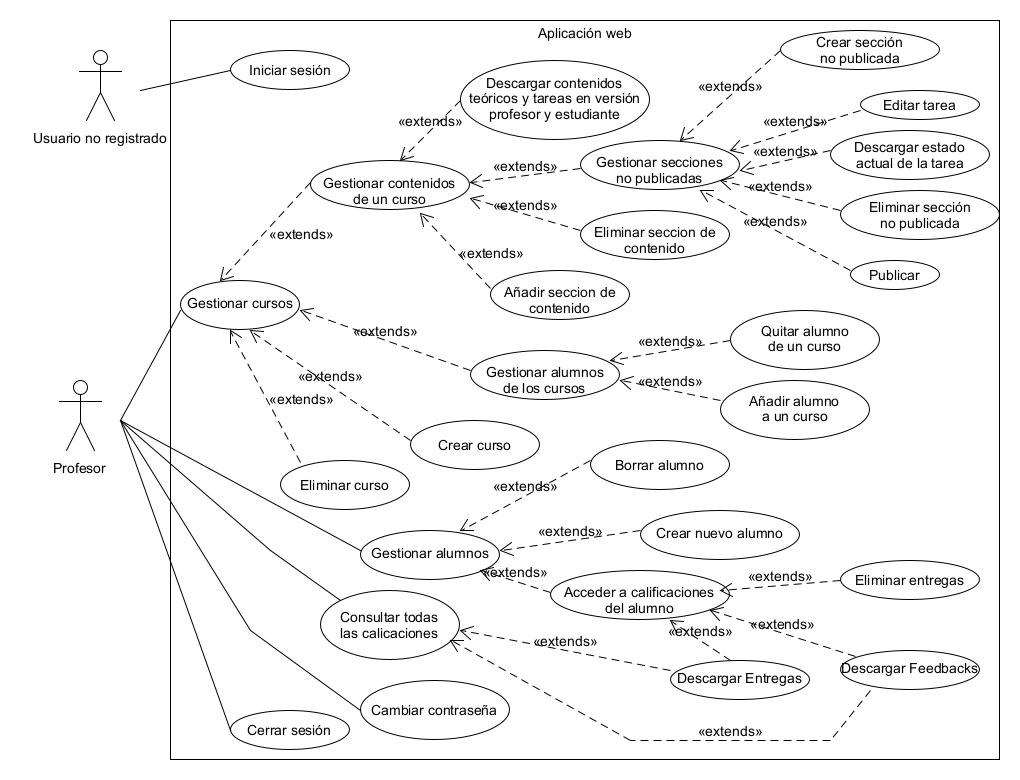
\includegraphics[width=\textwidth]{img/imgs-memoria/CasosDeUso_Profesor.png}
    \caption{Casos de Uso Profesor e Inicio de sesión}
\end{figure}

\begin{figure}[H]
    \centering
    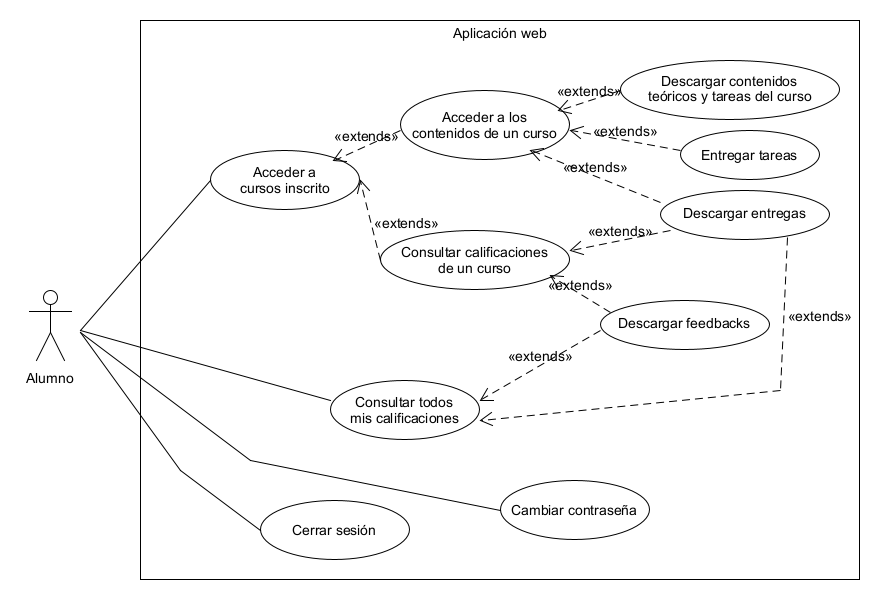
\includegraphics[width=\textwidth]{img/imgs-memoria/CasosDeUso_Alumno.png}
    \caption{Casos de Uso Alumno}
\end{figure}


\newpage
\subsection{Casos de uso}

\begin{adjustwidth}{-2cm}{}
\begin{tabular}[H]{l c l}
\toprule 
\multicolumn{3}{l}{\textbf{Caso de uso 1: Inicio de sesión}}\\
\midrule
Descripción & \multicolumn{2}{p{10cm}}{Permite a un usuario sin autenticar inciar sesión en la plataforma}\\
\midrule
Requisitos relacionados & \multicolumn{2}{p{10cm}}{RF-1}\\
\midrule
Precondiciones & \multicolumn{2}{p{10cm}}{El usuario dispone de una cuenta en la plataforma }\\
\midrule
Secuencia & Paso & Acción \\
\cmidrule{2-3}
         & 1 & El usuario accede al login de la plataforma \\
         & 2 & El usuario introduce su usuario y contraseña\\
         & 3 & Se inicia sesión\\
\midrule
Postcondiciones & \multicolumn{2}{p{10cm}}{El usuario es llevado a la página principal ''Inicio'' correspondiente en caso de ser un alumno o un profesor}\\
\midrule
Excepciones & \multicolumn{2}{p{10cm}}{Datos erróneos}\\
            & \multicolumn{2}{p{10cm}}{La cuenta no existe}\\
\bottomrule 
\end{tabular}


\hspace{3cm}

\begin{tabular}[H]{l c l}
\toprule 
\multicolumn{3}{l}{\textbf{Caso de uso 2: Gestionar cursos}}\\
\midrule
Descripción & \multicolumn{2}{p{10cm}}{Permite a un profesor realizar la gestión de sus cursos}\\
\midrule
Requisitos relacionados & \multicolumn{2}{p{10cm}}{RF-2, RF-2.1, RF-2.1.1, RF-2.1.2, RF-2.1.2.1, RF-2.1.2.2, RF-2.1.2.3
RF-2.1.2.4, RF-2.1.2.5, RF-2.1.3, RF-2.1.4, RF-2.2, RF-2.2.1, RF-2.2.2,  RF-2.3,  RF-2.4}\\
\midrule
Precondiciones & \multicolumn{2}{p{10cm}}{El profesor ha iniciado sesión}\\
\midrule
Secuencia & Paso & Acción \\
\cmidrule{2-3}
         & 1 & \multicolumn{1}{p{8cm}}{El profesor accede a la página de ''cursos'' desde la barra navegacional o desde el botón de ''cursos'' de la página principal ''Inicio''} \\
\midrule
Postcondiciones & \multicolumn{2}{p{10cm}}{El profesor es llevado a la página de gestión de sus cursos ''cursos''}\\
\bottomrule 
\end{tabular}
\end{adjustwidth}

\hspace{3cm}

\begin{tabular}[H]{l c l}
\toprule 
\multicolumn{3}{l}{\textbf{Caso de uso 2.1: Gestionar contenidos de un curso}}\\
\midrule
Descripción & \multicolumn{2}{p{10cm}}{Permite a un profesor realizar la gestión de contenidos de un curso en particular}\\
\midrule
Requisitos relacionados & \multicolumn{2}{p{10cm}}{RF-2, RF-2.1, RF-2.1.1, RF-2.1.2, RF-2.1.2.1, RF-2.1.2.2, RF-2.1.2.3
RF-2.1.2.4, RF-2.1.2.5, RF-2.1.3, RF-2.1.4}\\
\midrule
Precondiciones & \multicolumn{2}{p{10cm}}{El profesor ha accedido a la vista de gestión de cursos y el curso existe}\\
\midrule
Secuencia & Paso & Acción \\
\cmidrule{2-3}
         & 1 &  \multicolumn{1}{p{8cm}}{El profesor hace click en el botón ''Acceder'' del curso del cual quiere hacer la gestión de contenidos}\\

\midrule
Postcondiciones & \multicolumn{2}{p{10cm}}{El profesor es llevado a la página de contenidos del curso en particular}\\
\midrule
Excepciones & \multicolumn{2}{p{10cm}}{El curso no existe}\\
\bottomrule 
\end{tabular}

\hspace{3cm}


\begin{tabular}[H]{l c l}
\toprule 
\multicolumn{3}{l}{\textbf{Caso de uso 2.1.1: Descargar contenidos y tareas}}\\
\midrule
Descripción & \multicolumn{2}{p{10cm}}{Permite a un profesor descargar los archivos de contenidos teóricos y tareas de las secciones de contenido del curso actual }\\
\midrule
Requisitos relacionados & \multicolumn{2}{p{10cm}}{RF-2, RF-2.1, RF-2.1.2, RF-2.1.2.1, RF-2.1.2.2, RF-2.1.2.3
RF-2.1.2.4, RF-2.1.2.5}\\
\midrule
Precondiciones & \multicolumn{2}{p{10cm}}{El profesor ha accedido a la vista de contenidos de un curso}\\
\midrule
Secuencia & Paso & Acción \\
\cmidrule{2-3}
         & 1 &  \multicolumn{1}{p{8cm}}{El profesor hace click en los botones de descarga de contenidos teóricos y tareas de las secciones del curso}\\
\midrule
Postcondiciones & \multicolumn{2}{p{10cm}}{El profesor recibe los archivos que ha solicitado descargar}\\
\midrule
Excepciones & \multicolumn{2}{p{10cm}}{La sección no existe}\\
\bottomrule 
\end{tabular}

\hspace{3cm}

\begin{adjustwidth}{-2cm}{}
\begin{tabular}[H]{l c l}
\toprule 
\multicolumn{3}{l}{\textbf{Caso de uso 2.1.2: Gestionar secciones no publicadas}}\\
\midrule
Descripción & \multicolumn{2}{p{10cm}}{Permite a un profesor realizar la gestión de secciones de contenidos no publicadas de un curso }\\
\midrule
Requisitos relacionados & \multicolumn{2}{p{10cm}}{RF-2, RF-2.1, RF-2.1.2, RF-2.1.2.1, RF-2.1.2.2, RF-2.1.2.3
RF-2.1.2.4, RF-2.1.2.5}\\
\midrule
Precondiciones & \multicolumn{2}{p{10cm}}{El profesor ha accedido a la vista de contenidos de un curso}\\
\midrule
Secuencia & Paso & Acción \\
\cmidrule{2-3}
         & 1 &  \multicolumn{1}{p{8cm}}{El profesor hace click en el botón de acceso a las secciones no publicadas del curso}\\
\midrule
Postcondiciones & \multicolumn{2}{p{10cm}}{El profesor es llevado a la página de secciones no publicadas del curso actual}\\
\bottomrule 
\end{tabular}

\hspace{3cm}

\begin{tabular}[H]{l c l}
\toprule 
\multicolumn{3}{l}{\textbf{Caso de uso 2.1.2.1: Crear sección no publicada}}\\
\midrule
Descripción & \multicolumn{2}{p{10cm}}{Permite a un profesor crear una nueva sección no publicada en el curso actual}\\
\midrule
Requisitos relacionados & \multicolumn{2}{p{10cm}}{RF-2, RF-2.1, RF-2.1.2, RF-2.1.2.1}\\
\midrule
Precondiciones & \multicolumn{2}{p{10cm}}{El profesor ha accedido a la vista de contenidos de un curso o a la vista de secciones no publicadas de ese curso}\\
\midrule
Secuencia & Paso & Acción \\
\cmidrule{2-3}
         & 1 &  \multicolumn{1}{p{8cm}}{El profesor hace click en el botón de creación de sección no publicadas desde la vista del curso o la vista de secciones no publicadas del curso}\\
\midrule
Postcondiciones & \multicolumn{2}{p{10cm}}{Es creada una nueva sección no publicada y aparecerá en la vista de secciones no publicadas del curso}\\
\midrule
Excepciones & \multicolumn{2}{p{10cm}}{Información necesaria no aportada}\\
            & \multicolumn{2}{p{10cm}}{Contenidos pertenecientes a otra sección}\\
\bottomrule 
\end{tabular}
\end{adjustwidth}
\hspace{3cm}


\begin{tabular}[H]{l c l}
\toprule 
\multicolumn{3}{l}{\textbf{Caso de uso 2.1.2.2: Editar tarea}}\\
\midrule
Descripción & \multicolumn{2}{p{10cm}}{Permite a un profesor editar la tarea de una sección no publicada}\\
\midrule
Requisitos relacionados & \multicolumn{2}{p{10cm}}{RF-2, RF-2.1, RF-2.1.2, RF-2.1.2.2}\\
\midrule
Precondiciones & \multicolumn{2}{p{10cm}}{El profesor ha accedido a la vista de secciones no publicadas de ese curso}\\
\midrule
Secuencia & Paso & Acción \\
\cmidrule{2-3}
         & 1 &  \multicolumn{1}{p{8cm}}{El profesor hace click en el botón edición de tarea de una sección no publicada}\\
         & 2 &  \multicolumn{1}{p{8cm}}{El profesor edita la tarea desde la vista del notebook tarea que es abierta al realizar el paso anterior}\\
         & 3 &  \multicolumn{1}{p{8cm}}{El profesor guarda los cambios en el botón de guardado del notebook}\\
\midrule
Postcondiciones & \multicolumn{2}{p{10cm}}{La tarea es editada}\\
\midrule
Excepciones & \multicolumn{2}{p{10cm}}{La sección no publicada no existe}\\
\bottomrule 
\end{tabular}

\hspace{3cm}


\begin{tabular}[H]{l c l}
\toprule 
\multicolumn{3}{l}{\textbf{Caso de uso 2.1.2.3: Descargar estado de la tarea}}\\
\midrule
Descripción & \multicolumn{2}{p{10cm}}{Permite a un profesor descargar el estado actual de las tareas de las secciones no publicadas}\\
\midrule
Requisitos relacionados & \multicolumn{2}{p{10cm}}{RF-2, RF-2.1, RF-2.1.2, RF-2.1.2.3}\\
\midrule
Precondiciones & \multicolumn{2}{p{10cm}}{El profesor ha accedido a la vista de secciones no publicadas de ese curso}\\
\midrule
Secuencia & Paso & Acción \\
\cmidrule{2-3}
         & 1 &  \multicolumn{1}{p{8cm}}{El profesor hace click en el botón de descarga de la tarea de una sección no publicada}\\

\midrule
Postcondiciones & \multicolumn{2}{p{10cm}}{El profesor recibe el notebook tarea seleccionado}\\
\midrule
Excepciones & \multicolumn{2}{p{10cm}}{La sección no publicada no existe}\\
\bottomrule 
\end{tabular}

\hspace{3cm}

\begin{adjustwidth}{-2cm}{}
\begin{tabular}[H]{l c l}
\toprule 
\multicolumn{3}{l}{\textbf{Caso de uso 2.1.2.4: Eliminar sección no publicada}}\\
\midrule
Descripción & \multicolumn{2}{p{10cm}}{Permite a un profesor eliminar secciones no publicadas}\\
\midrule
Requisitos relacionados & \multicolumn{2}{p{10cm}}{RF-2, RF-2.1, RF-2.1.2, RF-2.1.2.4}\\
\midrule
Precondiciones & \multicolumn{2}{p{10cm}}{El profesor ha accedido a la vista de secciones no publicadas de ese curso}\\
\midrule
Secuencia & Paso & Acción \\
\cmidrule{2-3}
         & 1 &  \multicolumn{1}{p{8cm}}{El profesor hace click en el botón de eliminación de una sección no publicada}\\
         & 2 &  \multicolumn{1}{p{8cm}}{El profesor hace click en el botón de confirmación del modal emergente}\\
\midrule
Postcondiciones & \multicolumn{2}{p{10cm}}{La sección no publicada es eliminada}\\
\midrule
Excepciones & \multicolumn{2}{p{10cm}}{La sección no publicada no existe}\\
\bottomrule 
\end{tabular}

\hspace{3cm}

\begin{tabular}[H]{l c l}
\toprule 
\multicolumn{3}{l}{\textbf{Caso de uso 2.1.2.5: Publicar sección no publicada}}\\
\midrule
Descripción & \multicolumn{2}{p{10cm}}{Permite a un profesor publicar secciones no publicadas}\\
\midrule
Requisitos relacionados & \multicolumn{2}{p{10cm}}{RF-2, RF-2.1, RF-2.1.2, RF-2.1.2.5}\\
\midrule
Precondiciones & \multicolumn{2}{p{10cm}}{El profesor ha accedido a la vista de secciones no publicadas de ese curso}\\
\midrule
Secuencia & Paso & Acción \\
\cmidrule{2-3}
         & 1 &  \multicolumn{1}{p{8cm}}{El profesor hace click en el botón de publicación de una sección no publicada}\\
         & 2 &  \multicolumn{1}{p{8cm}}{El profesor hace click en el botón de confirmación del modal emergente}\\

\midrule
Postcondiciones & \multicolumn{2}{p{10cm}}{La sección no publicada es publicada, aparecerá en la vista de contenido del curso y se genera el archivo tarea correspondiente a esa sección para los alumnos}\\
\midrule
Excepciones & \multicolumn{2}{p{10cm}}{La sección no publicada no existe}\\
\bottomrule 
\end{tabular}
\end{adjustwidth}

\hspace{3cm}

\begin{tabular}[H]{l c l}
\toprule 
\multicolumn{3}{l}{\textbf{Caso de uso 2.1.3: Eliminar seccion de contenido}}\\
\midrule
Descripción & \multicolumn{2}{p{10cm}}{Permite a un profesor eliminar secciones de contenido del curso actual }\\
\midrule
Requisitos relacionados & \multicolumn{2}{p{10cm}}{RF-2, RF-2.1, RF-2.1.3}\\
\midrule
Precondiciones & \multicolumn{2}{p{10cm}}{El profesor ha accedido a la vista de contenidos de un curso}\\
\midrule
Secuencia & Paso & Acción \\
\cmidrule{2-3}
         & 1 &  \multicolumn{1}{p{8cm}}{El profesor hace click en el botón de eliminación de una sección de contenido del curso}\\
         & 2 &  \multicolumn{1}{p{8cm}}{El profesor hace click en el botón de confirmación del modal emergente}\\
         
\midrule
Postcondiciones & \multicolumn{2}{p{10cm}}{La sección de contenido es eliminada}\\
\midrule
Excepciones & \multicolumn{2}{p{10cm}}{La sección no existe}\\
\bottomrule 
\end{tabular}

\hspace{3cm}


\begin{tabular}[H]{l c l}
\toprule 
\multicolumn{3}{l}{\textbf{Caso de uso 2.1.4: Eliminar seccion de contenido}}\\
\midrule
Descripción & \multicolumn{2}{p{10cm}}{Permite a un profesor crear una sección de contenido de forma directa}\\
\midrule
Requisitos relacionados & \multicolumn{2}{p{10cm}}{RF-2, RF-2.1, RF-2.1.4}\\
\midrule
Precondiciones & \multicolumn{2}{p{10cm}}{El profesor ha accedido a la vista de contenidos de un curso}\\
\midrule
Secuencia & Paso & Acción \\
\cmidrule{2-3}
         & 1 &  \multicolumn{1}{p{8cm}}{El profesor hace click en el botón de creación de sección de contenido y es llevado a la vista de creación de sección}\\
         & 2 &  \multicolumn{1}{p{8cm}}{El profesor completa el formulario de creación de sección en el que introducirá el archivo de contenido teórico de la sección y el notebook tarea correspondiente a esa sección}\\
         & 3 &  \multicolumn{1}{p{8cm}}{El profesor hace click en el botón de crear}\\
         & 4 &  \multicolumn{1}{p{8cm}}{El profesor hace click en el botón de confirmación del modal emergente}\\
         
\midrule
Postcondiciones & \multicolumn{2}{p{10cm}}{La sección de contenido es creada y se genera el archivo tarea correspondiente a esa sección para los alumnos}\\
\bottomrule 
\end{tabular}

\hspace{3cm}

\begin{adjustwidth}{-2cm}{}
\begin{tabular}[H]{l c l}
\toprule 
\multicolumn{3}{l}{\textbf{Caso de uso 2.2: Gestionar alumnos de un curso}}\\
\midrule
Descripción & \multicolumn{2}{p{10cm}}{Permite a un profesor realizar la gestión de alumnos integrantes de un curso en particular}\\
\midrule
Requisitos relacionados & \multicolumn{2}{p{10cm}}{RF-2, RF-2.2, RF-2.2.1, RF-2.2.2}\\
\midrule
Precondiciones & \multicolumn{2}{p{10cm}}{El profesor ha accedido a la vista de gestión de cursos y el curso existe}\\
\midrule
Secuencia & Paso & Acción \\
\cmidrule{2-3}
         & 1 &  \multicolumn{1}{p{8cm}}{El profesor hace click en el botón de gestión de estudiantes del curso del cual quiere realizar la gestión}\\

\midrule
Postcondiciones & \multicolumn{2}{p{10cm}}{El profesor es llevado a la página de estudiantes integrantes y no integrantes del curso en particular}\\
\midrule
Excepciones & \multicolumn{2}{p{10cm}}{El curso no existe}\\
\bottomrule 
\end{tabular}

\hspace{3cm}

\begin{tabular}[H]{l c l}
\toprule 
\multicolumn{3}{l}{\textbf{Caso de uso 2.2.1: Quitar alumno de un curso}}\\
\midrule
Descripción & \multicolumn{2}{p{10cm}}{Permite a un profesor sacar a un alumno del curso actual}\\
\midrule
Requisitos relacionados & \multicolumn{2}{p{10cm}}{RF-2, RF-2.2, RF-2.2.1}\\
\midrule
Precondiciones & \multicolumn{2}{p{10cm}}{El profesor ha accedido a la vista de estudiantes integrantes y no integrantes del curso en particular}\\
\midrule
Secuencia & Paso & Acción \\
\cmidrule{2-3}
         & 1 &  \multicolumn{1}{p{8cm}}{El profesor hace click en el botón de extracción de un alumno del curso}\\
         & 2 &  \multicolumn{1}{p{8cm}}{El profesor hace click en el botón de confirmación del modal emergente}\\
\midrule
Postcondiciones & \multicolumn{2}{p{10cm}}{El alumno es extraido del curso}\\
\midrule
Excepciones & \multicolumn{2}{p{10cm}}{El alumno no pertenecía al curso}\\
\bottomrule 
\end{tabular}
\end{adjustwidth}


\hspace{3cm}

\begin{tabular}[H]{l c l}
\toprule 
\multicolumn{3}{l}{\textbf{Caso de uso 2.2.2: Añadir alumno a un curso}}\\
\midrule
Descripción & \multicolumn{2}{p{10cm}}{Permite a un profesor añadir a un alumno al curso actual}\\
\midrule
Requisitos relacionados & \multicolumn{2}{p{10cm}}{RF-2, RF-2.2, RF-2.2.2}\\
\midrule
Precondiciones & \multicolumn{2}{p{10cm}}{El profesor ha accedido a la vista de estudiantes integrantes y no integrantes del curso en particular}\\
\midrule
Secuencia & Paso & Acción \\
\cmidrule{2-3}
         & 1 &  \multicolumn{1}{p{8cm}}{El profesor hace click en el botón de adición de un alumno al curso}\\
         & 2 &  \multicolumn{1}{p{8cm}}{El profesor hace click en el botón de confirmación del modal emergente}\\
\midrule
Postcondiciones & \multicolumn{2}{p{10cm}}{El alumno es añadido al curso}\\
\midrule
Excepciones & \multicolumn{2}{p{10cm}}{El alumno ya pertenecía al curso}\\
\bottomrule 
\end{tabular}

\hspace{3cm}

\begin{tabular}[H]{l c l}
\toprule 
\multicolumn{3}{l}{\textbf{Caso de uso 2.3: Crear curso}}\\
\midrule
Descripción & \multicolumn{2}{p{10cm}}{Permite a un profesor crear un nuevo curso}\\
\midrule
Requisitos relacionados & \multicolumn{2}{p{10cm}}{RF-2, RF-2.3}\\
\midrule
Precondiciones & \multicolumn{2}{p{10cm}}{El profesor ha accedido a la vista de gestión de cursos}\\
\midrule
Secuencia & Paso & Acción \\
\cmidrule{2-3}
         & 1 &  \multicolumn{1}{p{8cm}}{El profesor hace click en el botón de creación de un nuevo curso y es llevado a la vista de creación de curso}\\
         & 2 &  \multicolumn{1}{p{8cm}}{El profesor completa el formulario de creación de un curso}\\
         & 3 &  \multicolumn{1}{p{8cm}}{El profesor hace click en el botón de crear curso}\\
         & 4 &  \multicolumn{1}{p{8cm}}{El profesor hace click en el botón de confirmación del modal emergente}\\

\midrule
Postcondiciones & \multicolumn{2}{p{10cm}}{El curso es creado y visualizable en la vista de gestión de cursos}\\
\midrule
Excepciones & \multicolumn{2}{p{10cm}}{Información necesaria no aportada}\\
            & \multicolumn{2}{p{10cm}}{Contenidos pertenecientes a otro curso}\\
\bottomrule 
\end{tabular}

\hspace{3cm}

\begin{adjustwidth}{-2cm}{}
\begin{tabular}[H]{l c l}
\toprule 
\multicolumn{3}{l}{\textbf{Caso de uso 2.4: Eliminar curso}}\\
\midrule
Descripción & \multicolumn{2}{p{10cm}}{Permite a un profesor elimianr un curso}\\
\midrule
Requisitos relacionados & \multicolumn{2}{p{10cm}}{RF-2, RF-2.4}\\
\midrule
Precondiciones & \multicolumn{2}{p{10cm}}{El profesor ha accedido a la vista de gestión de cursos}\\
\midrule
Secuencia & Paso & Acción \\
\cmidrule{2-3}
         & 1 &  \multicolumn{1}{p{8cm}}{El profesor hace click en el botón de eliminación de un curso}\\
         & 2 &  \multicolumn{1}{p{8cm}}{El profesor hace click en el botón de confirmación del modal emergente}\\

\midrule
Postcondiciones & \multicolumn{2}{p{10cm}}{El curso es eliminado}\\
\midrule
Excepciones & \multicolumn{2}{p{10cm}}{El curso no existe}\\
\bottomrule 
\end{tabular}


\hspace{3cm}


\begin{tabular}[H]{l c l}
\toprule 
\multicolumn{3}{l}{\textbf{Caso de uso 3: Gestionar alumnos}}\\
\midrule
Descripción & \multicolumn{2}{p{10cm}}{Permite a un profesor realizar la gestión de alumnos pertenecientes a sus cursos}\\
\midrule
Requisitos relacionados & \multicolumn{2}{p{10cm}}{RF-3, RF-3.1, RF-3.2, RF-3.3, RF-3.3.1, RF-3.3.2, RF-3.3.3}\\
\midrule
Precondiciones & \multicolumn{2}{p{10cm}}{El profesor ha iniciado sesión}\\
\midrule
Secuencia & Paso & Acción \\
\cmidrule{2-3}
         & 1 & \multicolumn{1}{p{8cm}}{El profesor accede a la página de gestión de alumnos desde la barra navegacional o desde el botón de gestión de alumnos de la página principal} \\
\midrule
Postcondiciones & \multicolumn{2}{p{10cm}}{El profesor es llevado a la página de gestión de alumnos}\\
\bottomrule 
\end{tabular}
\end{adjustwidth}

\hspace{3cm}

\begin{tabular}[H]{l c l}
\toprule 
\multicolumn{3}{l}{\textbf{Caso de uso 3.1: Crear alumno}}\\
\midrule
Descripción & \multicolumn{2}{p{10cm}}{Permite a un profesor crear un nuevo alumno}\\
\midrule
Requisitos relacionados & \multicolumn{2}{p{10cm}}{RF-3, RF-3.1}\\
\midrule
Precondiciones & \multicolumn{2}{p{10cm}}{El profesor ha accedido a la vista de gestión de alumnos pertenecientes a sus cursos}\\
\midrule
Secuencia & Paso & Acción \\
\cmidrule{2-3}
         & 1 &  \multicolumn{1}{p{8cm}}{El profesor hace click en el botón de creación de un nuevo alumno y es llevado a la vista de creación de alumno}\\
         & 2 &  \multicolumn{1}{p{8cm}}{El profesor completa el formulario de creación del alumno y selecciona un curso al que quiere ingresar al alumno}\\
         & 3 &  \multicolumn{1}{p{8cm}}{El profesor hace click en el botón de crear alumno}\\
         & 4 &  \multicolumn{1}{p{8cm}}{El profesor hace click en el botón de confirmación del modal emergente}\\

\midrule
Postcondiciones & \multicolumn{2}{p{10cm}}{El alumno es creado y visualizable en la vista de gestión de alumnos}\\
\midrule
Excepciones & \multicolumn{2}{p{10cm}}{Información necesaria no aportada}\\
            & \multicolumn{2}{p{10cm}}{Contenidos pertenecientes a otro alumno}\\
\bottomrule 
\end{tabular}

\hspace{3cm}

\begin{adjustwidth}{-2cm}{}
\begin{tabular}[H]{l c l}
\toprule 
\multicolumn{3}{l}{\textbf{Caso de uso 3.2: Borrar alumno}}\\
\midrule
Descripción & \multicolumn{2}{p{10cm}}{Permite a un profesor borrar un alumno}\\
\midrule
Requisitos relacionados & \multicolumn{2}{p{10cm}}{RF-3, RF-3.2}\\
\midrule
Precondiciones & \multicolumn{2}{p{10cm}}{El profesor ha accedido a la vista de gestión de alumnos pertenecientes a sus cursos}\\
\midrule
Secuencia & Paso & Acción \\
\cmidrule{2-3}
         & 1 &  \multicolumn{1}{p{8cm}}{El profesor hace click en el nombre del estudiante accediendo al perfil este en el que se visualizan las calificaciones}\\
         & 2 &  \multicolumn{1}{p{8cm}}{El profesor hace click en el botón de eliminación del alumno}\\
         & 3 &  \multicolumn{1}{p{8cm}}{El profesor hace click en el botón de confirmación del modal emergente}\\

\midrule
Postcondiciones & \multicolumn{2}{p{10cm}}{El alumno es eliminado junto con su cuenta}\\
\midrule
Excepciones & \multicolumn{2}{p{10cm}}{El alumno no existe}\\
\bottomrule 
\end{tabular}

\hspace{3cm}

\begin{tabular}[H]{l c l}
\toprule 
\multicolumn{3}{l}{\textbf{Caso de uso 3.3: Acceder a las calificaciones de un alumno}}\\
\midrule
Descripción & \multicolumn{2}{p{10cm}}{Permite a un profesor visualizar todas las calificaciones de un alumno en particular}\\
\midrule
Requisitos relacionados & \multicolumn{2}{p{10cm}}{RF-3, RF-3.3, RF-3.3.1, RF-3.3.2,  RF-3.3.3}\\
\midrule
Precondiciones & \multicolumn{2}{p{10cm}}{El profesor ha accedido a la vista de gestión de alumnos pertenecientes a sus cursos}\\
\midrule
Secuencia & Paso & Acción \\
\cmidrule{2-3}
         & 1 &  \multicolumn{1}{p{8cm}}{El profesor hace click en el nombre del estudiante accediendo al perfil este en el que se visualizan las calificaciones}\\

\midrule
Postcondiciones & \multicolumn{2}{p{10cm}}{El profesor visualiza las calificaciones}\\
\midrule
Excepciones & \multicolumn{2}{p{10cm}}{El alumno no existe}\\
\bottomrule 
\end{tabular}
\end{adjustwidth}


\hspace{3cm}


\begin{tabular}[H]{l c l}
\toprule 
\multicolumn{3}{l}{\textbf{Caso de uso 3.3.1: Eliminar entregas}}\\
\midrule
Descripción & \multicolumn{2}{p{10cm}}{Permite a un profesor eliminar entregas / calificaciones de tareas realizadas por un alumno en particular}\\
\midrule
Requisitos relacionados & \multicolumn{2}{p{10cm}}{RF-3, RF-3.3, RF-3.3.1}\\
\midrule
Precondiciones & \multicolumn{2}{p{10cm}}{El profesor ha accedido a la vista de gestión de alumnos pertenecientes a sus cursos}\\
\midrule
Secuencia & Paso & Acción \\
\cmidrule{2-3}
         & 1 &  \multicolumn{1}{p{8cm}}{El profesor hace click en el nombre del estudiante accediendo al perfil este en el que se visualizan las calificaciones}\\
         & 2 &  \multicolumn{1}{p{8cm}}{El profesor hace click en el botón de eliminación de entrega de una calificación en particular}\\
         & 3 &  \multicolumn{1}{p{8cm}}{El profesor hace click en el botón de confirmación del modal emergente}\\
\midrule
Postcondiciones & \multicolumn{2}{p{10cm}}{El profesor elimina la entrega}\\
\midrule
Excepciones & \multicolumn{2}{p{10cm}}{La calificación no existe}\\
\bottomrule 
\end{tabular}

\hspace{3cm}

\begin{tabular}[H]{l c l}
\toprule 
\multicolumn{3}{l}{\textbf{Caso de uso 3.3.2: Descargar feedback}}\\
\midrule
Descripción & \multicolumn{2}{p{10cm}}{Permite a un profesor descargar los archivos de feedback de las entregas / calificaciones de un alumno en particular}\\
\midrule
Requisitos relacionados & \multicolumn{2}{p{10cm}}{RF-3, RF-3.3, RF-3.3.2}\\
\midrule
Precondiciones & \multicolumn{2}{p{10cm}}{El profesor ha accedido a la vista de gestión de alumnos pertenecientes a sus cursos}\\
\midrule
Secuencia & Paso & Acción \\
\cmidrule{2-3}
         & 1 &  \multicolumn{1}{p{8cm}}{El profesor hace click en el nombre del estudiante accediendo al perfil este en el que se visualizan las calificaciones}\\
         & 2 &  \multicolumn{1}{p{8cm}}{El profesor hace click en el botón de descarga de feedback de una calificación en particular}\\

\midrule
Postcondiciones & \multicolumn{2}{p{10cm}}{El profesor recibe el archivo feedback}\\
\midrule
Excepciones & \multicolumn{2}{p{10cm}}{La calificación no existe}\\
\bottomrule 
\end{tabular}

\hspace{3cm}

\begin{adjustwidth}{-2cm}{}
\begin{tabular}[H]{l c l}
\toprule 
\multicolumn{3}{l}{\textbf{Caso de uso 3.3.3: Descargar entregas}}\\
\midrule
Descripción & \multicolumn{2}{p{10cm}}{Permite a un profesor descargar los archivos entregados de las entregas / calificaciones de un alumno en particular}\\
\midrule
Requisitos relacionados & \multicolumn{2}{p{10cm}}{RF-3, RF-3.3, RF-3.3.3}\\
\midrule
Precondiciones & \multicolumn{2}{p{10cm}}{El profesor ha accedido a la vista de gestión de alumnos pertenecientes a sus cursos}\\
\midrule
Secuencia & Paso & Acción \\
\cmidrule{2-3}
         & 1 &  \multicolumn{1}{p{8cm}}{El profesor hace click en el nombre del estudiante accediendo al perfil este en el que se visualizan las calificaciones}\\
         & 2 &  \multicolumn{1}{p{8cm}}{El profesor hace click en el botón de descarga de entrega de una calificación en particular}\\

\midrule
Postcondiciones & \multicolumn{2}{p{10cm}}{El profesor recibe el archivo de entrega del alumno}\\
\midrule
Excepciones & \multicolumn{2}{p{10cm}}{La calificación no existe}\\
\bottomrule 
\end{tabular}

\hspace{3cm} 

\begin{tabular}[H]{l c l}
\toprule 
\multicolumn{3}{l}{\textbf{Caso de uso 4: Consultar todas las calificaciones}}\\
\midrule
Descripción & \multicolumn{2}{p{10cm}}{Permite a un profesor acceder a todas las calificaciones de todos los alumnos pertenecientes a sus cursos}\\
\midrule
Requisitos relacionados & \multicolumn{2}{p{10cm}}{RF-4, RF-4.1, RF-4.2}\\
\midrule
Precondiciones & \multicolumn{2}{p{10cm}}{El profesor ha iniciado sesión}\\
\midrule
Secuencia & Paso & Acción \\
\cmidrule{2-3}
         & 1 & \multicolumn{1}{p{8cm}}{El profesor accede a la página de calificaciones desde la barra navegacional o desde el botón de calificaciones de la página principal} \\
\midrule
Postcondiciones & \multicolumn{2}{p{10cm}}{El profesor es llevado a la página de calificaciones}\\
\bottomrule 
\end{tabular}
\end{adjustwidth}


\hspace{3cm} 

\begin{tabular}[H]{l c l}
\toprule 
\multicolumn{3}{l}{\textbf{Caso de uso 4.1: Descargar feedback}}\\
\midrule
Descripción & \multicolumn{2}{p{10cm}}{Permite a un profesor descargar los archivos de feedback de las entregas / calificaciones de sus alumnos}\\
\midrule
Requisitos relacionados & \multicolumn{2}{p{10cm}}{RF-4, RF-4.1}\\
\midrule
Precondiciones & \multicolumn{2}{p{10cm}}{El profesor ha accedido a la vista de calificaciones}\\
\midrule
Secuencia & Paso & Acción \\
\cmidrule{2-3}
         & 1 &  \multicolumn{1}{p{8cm}}{El profesor hace click en el botón de descarga de feedback de una calificación en particular}\\
\midrule
Postcondiciones & \multicolumn{2}{p{10cm}}{El profesor recibe el archivo feedback}\\
\midrule
Excepciones & \multicolumn{2}{p{10cm}}{La calificación no existe}\\
\bottomrule 
\end{tabular}



\hspace{3cm} 


\begin{tabular}[H]{l c l}
\toprule 
\multicolumn{3}{l}{\textbf{Caso de uso 4.2: Descargar entregas}}\\
\midrule
Descripción & \multicolumn{2}{p{10cm}}{Permite a un profesor descargar los archivos entregados de las entregas / calificaciones de sus alumnos}\\
\midrule
Requisitos relacionados & \multicolumn{2}{p{10cm}}{RF-4, RF-4.2}\\
\midrule
Precondiciones & \multicolumn{2}{p{10cm}}{El profesor ha accedido a la vista de calificaciones}\\
\midrule
Secuencia & Paso & Acción \\
\cmidrule{2-3}
         & 1 &  \multicolumn{1}{p{8cm}}{El profesor hace click en el botón de descarga de entrega de una calificación en particular}\\
\midrule
Postcondiciones & \multicolumn{2}{p{10cm}}{El profesor recibe el archivo de entrega del alumno}\\
\midrule
Excepciones & \multicolumn{2}{p{10cm}}{La calificación no existe}\\
\bottomrule 
\end{tabular}

\hspace{3cm} 


\begin{adjustwidth}{-2cm}{}
\begin{tabular}[H]{l c l}
\toprule 
\multicolumn{3}{l}{\textbf{Caso de uso 5: Acceder a cursos inscrito}}\\
\midrule
Descripción & \multicolumn{2}{p{10cm}}{Permite a un alumno acceder a los cursos a los que está inscrito}\\
\midrule
Requisitos relacionados & \multicolumn{2}{p{10cm}}{RF-5, RF-5.1, RF-5.1.1, RF-5.1.2, RF-5.1.3}\\
\midrule
Precondiciones & \multicolumn{2}{p{10cm}}{El alumno ha iniciado sesión}\\
\midrule
Secuencia & Paso & Acción \\
\cmidrule{2-3}
         & 1 & \multicolumn{1}{p{8cm}}{El alumno accede a la página de cursos desde la barra navegacional o desde el botón de cursos de la página principal} \\
\midrule
Postcondiciones & \multicolumn{2}{p{10cm}}{El alumno es llevado a la página de cursos}\\
\bottomrule 
\end{tabular}


\hspace{3cm} 

\begin{tabular}[H]{l c l}
\toprule 
\multicolumn{3}{l}{\textbf{Caso de uso 5.1: Acceder a contenidos de un curso}}\\
\midrule
Descripción & \multicolumn{2}{p{10cm}}{Permite a un alumno realizar acceder a los contenidos de un curso en particular}\\
\midrule
Requisitos relacionados & \multicolumn{2}{p{10cm}}{RF-5, RF-5.1, RF-5.1.1,  RF-5.1.2, RF-5.1.3}\\
\midrule
Precondiciones & \multicolumn{2}{p{10cm}}{El alumno ha accedido a la vista de cursos y el curso existe}\\
\midrule
Secuencia & Paso & Acción \\
\cmidrule{2-3}
         & 1 &  \multicolumn{1}{p{8cm}}{El alumno hace click en el botón de acceso al curso}\\

\midrule
Postcondiciones & \multicolumn{2}{p{10cm}}{El alumno es llevado a la página de contenidos del curso en particular}\\
\midrule
Excepciones & \multicolumn{2}{p{10cm}}{El curso no existe}\\
\bottomrule 
\end{tabular}
\end{adjustwidth}

\hspace{3cm} 

\begin{tabular}[H]{l c l}
\toprule 
\multicolumn{3}{l}{\textbf{Caso de uso 5.1.1: Descargar contenidos y tareas}}\\
\midrule
Descripción & \multicolumn{2}{p{10cm}}{Permite a un alumno descargarse los contenidos teóricos y tareas de las secciones pertenecientes al curso en particular}\\
\midrule
Requisitos relacionados & \multicolumn{2}{p{10cm}}{RF-5, RF-5.1, RF-5.1.1}\\
\midrule
Precondiciones & \multicolumn{2}{p{10cm}}{El alumno ha accedido a la vista del curso y la sección de contenido existe}\\
\midrule
Secuencia & Paso & Acción \\
\cmidrule{2-3}
         & 1 &  \multicolumn{1}{p{8cm}}{El alumno hace click los botones de descarga de contenido teórico y tareas de la sección en particular de la que quiere obtener los archivos}\\

\midrule
Postcondiciones & \multicolumn{2}{p{10cm}}{El alumno recibe los archivos pedidos}\\
\midrule
Excepciones & \multicolumn{2}{p{10cm}}{La sección de contenido no existe}\\
\bottomrule 
\end{tabular}

\hspace{3cm} 

\begin{tabular}[H]{l c l}
\toprule 
\multicolumn{3}{l}{\textbf{Caso de uso 5.1.2: Entregar tareas}}\\
\midrule
Descripción & \multicolumn{2}{p{10cm}}{Permite a un alumno realizar la entrega de tareas de un curso}\\
\midrule
Requisitos relacionados & \multicolumn{2}{p{10cm}}{RF-5, RF-5.1, RF-5.1.2}\\
\midrule
Precondiciones & \multicolumn{2}{p{10cm}}{El alumno ha accedido a la vista del curso y la sección de contenido existe}\\
\midrule
Secuencia & Paso & Acción \\
\cmidrule{2-3}
         & 1 &  \multicolumn{1}{p{8cm}}{El alumno hace click en el botón de exploración de archivos de la sección de contenido en la que quiere entregar la tarea}\\
         & 2 &  \multicolumn{1}{p{8cm}}{El alumno hace click en el botón de entrega de la tarea}\\
         
\midrule
Postcondiciones & \multicolumn{2}{p{10cm}}{La entrega es realizada, la calificación es calculada y el archivo de feedback es generado}\\
\midrule
Excepciones & \multicolumn{2}{p{10cm}}{La sección de contenido no existe}\\
            & \multicolumn{2}{p{10cm}}{La tarea ya ha sido entregada previamente}\\
\bottomrule 
\end{tabular}

\hspace{3cm}

\begin{adjustwidth}{-2cm}{}
\begin{tabular}[H]{l c l}
\toprule 
\multicolumn{3}{l}{\textbf{Caso de uso 5.1.3: Descargar entregas}}\\
\midrule
Descripción & \multicolumn{2}{p{10cm}}{Permite a un alumno descargar las entregas de las tareas previamente entregadas desde la propia vista del curso}\\
\midrule
Requisitos relacionados & \multicolumn{2}{p{10cm}}{RF-5, RF-5.1, RF-5.1.3}\\
\midrule
Precondiciones & \multicolumn{2}{p{10cm}}{El alumno ha accedido a la vista del curso y la sección de contenido existe y ha sido entregada su tarea}\\
\midrule
Secuencia & Paso & Acción \\
\cmidrule{2-3}
         & 1 &  \multicolumn{1}{p{8cm}}{El alumno hace click en el botón de descarga de la entrega en la sección correspondiente}\\
         
\midrule
Postcondiciones & \multicolumn{2}{p{10cm}}{El alumno recibe el archivo de entrega}\\
\midrule
Excepciones & \multicolumn{2}{p{10cm}}{La sección de contenido no existe}\\
            & \multicolumn{2}{p{10cm}}{La tarea no ha sido entregada}\\
\bottomrule 
\end{tabular}

\hspace{3cm}


\begin{tabular}[H]{l c l}
\toprule 
\multicolumn{3}{l}{\textbf{Caso de uso 5.2: Consultar calificaciones de un curso}}\\
\midrule
Descripción & \multicolumn{2}{p{10cm}}{Permite a un alumno consultar las calificaciones obtenidas en un curso en particular}\\
\midrule
Requisitos relacionados & \multicolumn{2}{p{10cm}}{RF-5, RF-5.2, RF-5.2.1,  RF-5.2.2}\\
\midrule
Precondiciones & \multicolumn{2}{p{10cm}}{El alumno ha accedido a la vista de cursos y el curso existe}\\
\midrule
Secuencia & Paso & Acción \\
\cmidrule{2-3}
         & 1 &  \multicolumn{1}{p{8cm}}{El alumno hace click en el botón de calificaciones del curso}\\

\midrule
Postcondiciones & \multicolumn{2}{p{10cm}}{El alumno es llevado a la página de calificaciones del curso en particular}\\
\midrule
Excepciones & \multicolumn{2}{p{10cm}}{El curso no existe}\\
\bottomrule 
\end{tabular}
\end{adjustwidth}

\hspace{3cm}

\begin{tabular}[H]{l c l}
\toprule 
\multicolumn{3}{l}{\textbf{Caso de uso 5.2.1: Descargar entregas}}\\
\midrule
Descripción & \multicolumn{2}{p{10cm}}{Permite a un alumno descargar las entregas de las tareas previamente entregadas desde la vista de calificaciones de un curso particular}\\
\midrule
Requisitos relacionados & \multicolumn{2}{p{10cm}}{RF-5, RF-5.2, RF-5.2.1}\\
\midrule
Precondiciones & \multicolumn{2}{p{10cm}}{El alumno ha accedido a la vista de calificaciones de un curso particular}\\
\midrule
Secuencia & Paso & Acción \\
\cmidrule{2-3}
         & 1 &  \multicolumn{1}{p{8cm}}{El alumno hace click en el botón de descarga de entrega de una calificación en particular}\\
         
\midrule
Postcondiciones & \multicolumn{2}{p{10cm}}{El alumno recibe el archivo de entrega}\\
\midrule
Excepciones  & \multicolumn{2}{p{10cm}}{La calificación no existe}\\
\bottomrule 
\end{tabular}


\hspace{3cm}

\begin{tabular}[H]{l c l}
\toprule 
\multicolumn{3}{l}{\textbf{Caso de uso 5.2.2: Descargar feedback}}\\
\midrule
Descripción & \multicolumn{2}{p{10cm}}{Permite a un alumno descargar los archivos de feedback de las entregas / calificaciones desde la vista de calificaciones de un curso particular}\\
\midrule
Requisitos relacionados & \multicolumn{2}{p{10cm}}{RF-5, RF-5.2, RF-5.2.2}\\
\midrule
Precondiciones & \multicolumn{2}{p{10cm}}{El alumno ha accedido a la vista de calificaciones de un curso particular}\\
\midrule
Secuencia & Paso & Acción \\
\cmidrule{2-3}
         & 1 &  \multicolumn{1}{p{8cm}}{El alumno hace click en el botón de descarga de feedback de una calificación en particular}\\
         
\midrule
Postcondiciones & \multicolumn{2}{p{10cm}}{El alumno recibe el archivo de feedback}\\
\midrule
Excepciones  & \multicolumn{2}{p{10cm}}{La calificación no existe}\\
\bottomrule 
\end{tabular}


\hspace{3cm} 

\begin{adjustwidth}{-2cm}{}
\begin{tabular}[H]{l c l}
\toprule 
\multicolumn{3}{l}{\textbf{Caso de uso 6: Consultar todas mis calificaciones}}\\
\midrule
Descripción & \multicolumn{2}{p{10cm}}{Permite a un alumno consultar todas sus calificaciones obtenidas}\\
\midrule
Requisitos relacionados & \multicolumn{2}{p{10cm}}{RF-5, RF-5.1, RF-5.1.1, RF-5.1.2, RF-5.1.3}\\
\midrule
Precondiciones & \multicolumn{2}{p{10cm}}{El alumno ha iniciado sesión}\\
\midrule
Secuencia & Paso & Acción \\
\cmidrule{2-3}
         & 1 & \multicolumn{1}{p{8cm}}{El alumno accede a la página de calificaciones desde la barra navegacional o desde el botón de calificaciones de la página principal} \\
\midrule
Postcondiciones & \multicolumn{2}{p{10cm}}{El alumno es llevado a la página calificaciones}\\
\bottomrule 
\end{tabular}



\hspace{3cm}

\begin{tabular}[H]{l c l}
\toprule 
\multicolumn{3}{l}{\textbf{Caso de uso 6.1: Descargar entregas}}\\
\midrule
Descripción & \multicolumn{2}{p{10cm}}{Permite a un alumno descargar las entregas de las tareas previamente entregadas desde la vista de calificaciones}\\
\midrule
Requisitos relacionados & \multicolumn{2}{p{10cm}}{RF-6, RF-6.1}\\
\midrule
Precondiciones & \multicolumn{2}{p{10cm}}{El alumno ha accedido a la vista de todas sus calificaciones}\\
\midrule
Secuencia & Paso & Acción \\
\cmidrule{2-3}
         & 1 &  \multicolumn{1}{p{8cm}}{El alumno hace click en el botón de descarga de entrega de una calificación en particular}\\
         
\midrule
Postcondiciones & \multicolumn{2}{p{10cm}}{El alumno recibe el archivo de entrega}\\
\midrule
Excepciones  & \multicolumn{2}{p{10cm}}{La calificación no existe}\\
\bottomrule 
\end{tabular}
\end{adjustwidth}


\hspace{3cm}

\begin{tabular}[H]{l c l}
\toprule 
\multicolumn{3}{l}{\textbf{Caso de uso 6.2: Descargar feedback}}\\
\midrule
Descripción & \multicolumn{2}{p{10cm}}{Permite a un alumno descargar los archivos de feedback de las entregas / calificaciones desde la vista de todas sus calificaciones}\\
\midrule
Requisitos relacionados & \multicolumn{2}{p{10cm}}{RF-6, RF-6.2}\\
\midrule
Precondiciones & \multicolumn{2}{p{10cm}}{El alumno ha accedido a la vista de todas sus calificaciones}\\
\midrule
Secuencia & Paso & Acción \\
\cmidrule{2-3}
         & 1 &  \multicolumn{1}{p{8cm}}{El alumno hace click en el botón de descarga de feedback de una calificación en particular}\\
         
\midrule
Postcondiciones & \multicolumn{2}{p{10cm}}{El alumno recibe el archivo de feedback}\\
\midrule
Excepciones  & \multicolumn{2}{p{10cm}}{La calificación no existe}\\
\bottomrule 
\end{tabular}


\hspace{3cm}

\begin{tabular}[H]{l c l}
\toprule 
\multicolumn{3}{l}{\textbf{Caso de uso 7: Cambio de contraseña}}\\
\midrule
Descripción & \multicolumn{2}{p{10cm}}{Permite a un usuario (profesor o alumno) realizar el cambio de contraseña de su cuenta}\\
\midrule
Requisitos relacionados & \multicolumn{2}{p{10cm}}{RF-7}\\
\midrule
Precondiciones & \multicolumn{2}{p{10cm}}{El usuario ha iniciado sesión}\\
\midrule
Secuencia & Paso & Acción \\
\cmidrule{2-3}
         & 1 &  \multicolumn{1}{p{8cm}}{El usuario hace click en el botón de cambio de contraseña de la página principal y es llevado a la vista de cambio de contraseña}\\
         & 2 &  \multicolumn{1}{p{8cm}}{El usuario rellena el formulario de cambio de contraseña}\\
         & 3 &  \multicolumn{1}{p{8cm}}{El usuario hace click en el botón de cambio de contraseña}\\
         & 4 &  \multicolumn{1}{p{8cm}}{El usuario hace click en el botón de confirmación del modal emergente}\\
         
\midrule
Postcondiciones & \multicolumn{2}{p{10cm}}{La contraseña es cambiada y se produce un cierre de sesión llevandose al usuario al login}\\
\midrule
Excepciones  & \multicolumn{2}{p{10cm}}{Datos de entrada incorrectos}\\
\bottomrule 
\end{tabular}


\hspace{3cm}

\begin{adjustwidth}{-2cm}{}
\begin{tabular}[H]{l c l}
\toprule 
\multicolumn{3}{l}{\textbf{Caso de uso 8: Cierre de sesión}}\\
\midrule
Descripción & \multicolumn{2}{p{10cm}}{Permite a un usuario (profesor o alumno) realizar el cierre de sesión}\\
\midrule
Requisitos relacionados & \multicolumn{2}{p{10cm}}{RF-7}\\
\midrule
Precondiciones & \multicolumn{2}{p{10cm}}{El usuario ha iniciado sesión}\\
\midrule
Secuencia & Paso & Acción \\
\cmidrule{2-3}
         & 1 &  \multicolumn{1}{p{8cm}}{El usuario hace click en el botón de cierre de sesión de la página principal}\\
         & 2 &  \multicolumn{1}{p{8cm}}{El usuario hace click en el botón de confirmación del modal emergente}\\
         
\midrule
Postcondiciones & \multicolumn{2}{p{10cm}}{Se produce el cierre de sesión llevandose al usuario al login}\\
\bottomrule 
\end{tabular}
\end{adjustwidth}
\apendice{Especificación de diseño}

\section{Introducción}
En este anexo será descrito el diseño, el cual ha sido llevado a cabo en el desarrollo de la plataforma buscando los objetivos y funcionalidades descritos anteriormente. En concreto, viendo el diseño de datos, el diseño procedimental y el diseño arquitectónico.

\section{Diseño de datos}
Las entidades definidas para el funcionamiento de la plataforma y presentes en base de datos son las siguientes:

\begin{itemize}
\item Usuario (User): correspondiente a los usuarios del sistema los cuales pueden ser de tipo profesor o de tipo alumno. Cuentan con identificador, nombre, nombre de usuario, contraseña, campo de control de tipo de usuario y campo de control de primer inicio de sesión.

\item Curso (Course): correspondiente a los cursos del sistema. Cuenta con identificador, identificador del usuario profesor al que pertenece el curso, nombre y descripción 

\item Sección (Section): correspondiente a las secciones de los cursos. Cuenta con identificador, identificador del curso al que pertenece, nombre, nombre del archivo de contenido de la sección y nombre de la tarea de la sección.

\item Calificación (Calification): Correspondiente a las calificaciones de los alumnos. Cuenta con el identificador del estudiante al que pertenece, identificador de la sección a la que pertenece, nombre de la tarea y el valor obtenido.

\item Miembros del curso(Course Members): encargada de guardar las relaciones entre los cursos y los alumnos pertenecientes a estos. Cuenta con el identificador del curso y el del estudiante registrado en el curso.

\item Sección sin publicar (Unreleased Section): correspondiente a secciones no publicadas dedicadas a la creación de tareas de forma manual por los profesores desde la plataforma. Cuenta con identificador, identificador del profesor al que pertenecen, identificador del curso al que pertenecen, nombre, nombre del archivo de contenido de la sección y nombre de la tarea de la sección.


\subsubsection{Diagrama E/R}
\begin{figure}[H]
    \centering
    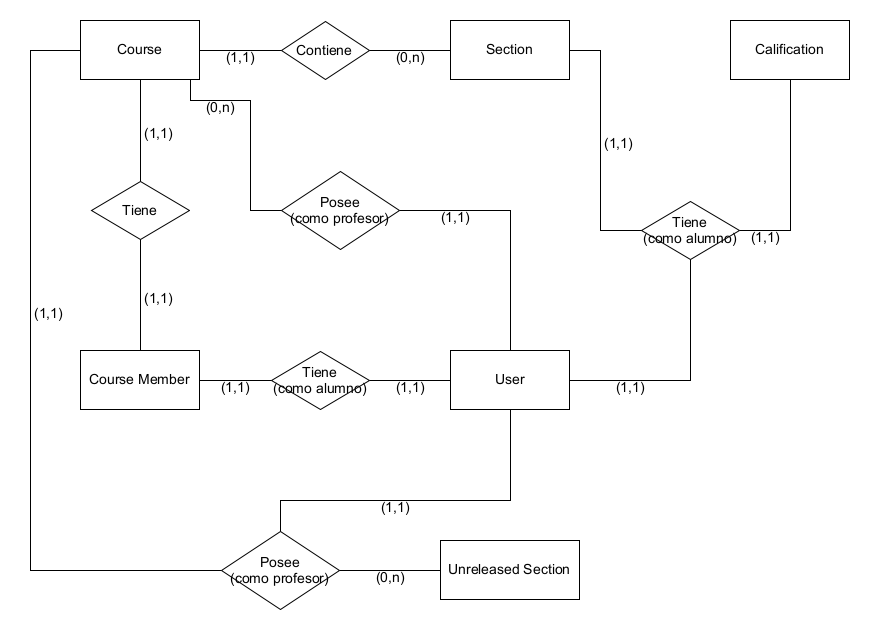
\includegraphics[width=\textwidth]{img/imgs-memoria/BD_DiagramaER.png}
    \caption{Diagrama E/R}
\end{figure}


\subsubsection{Diagrama Relacional}
\begin{figure}[H]
    \centering
    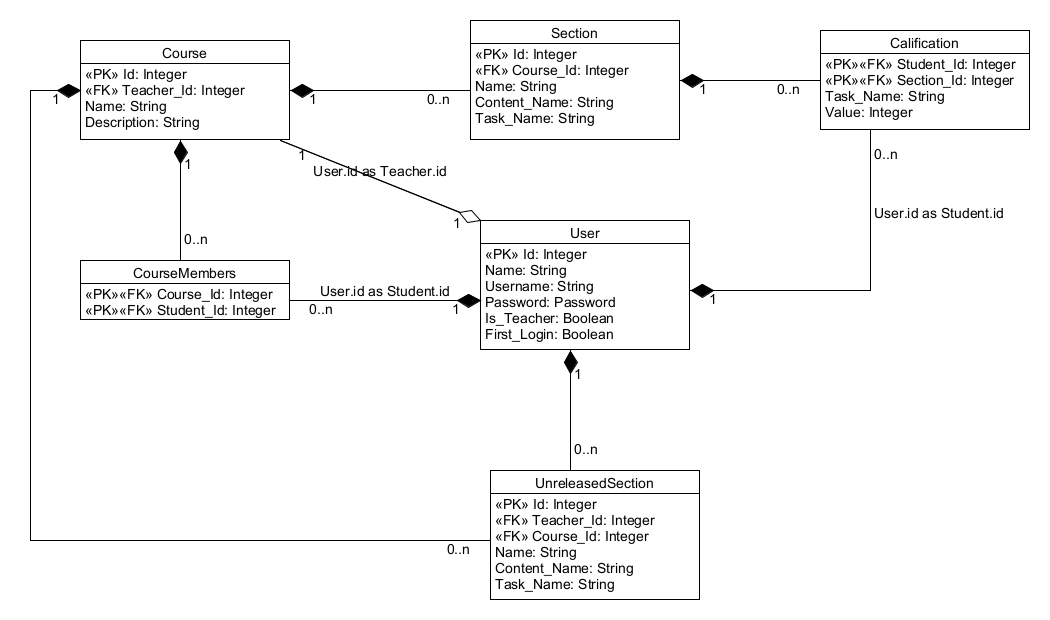
\includegraphics[width=\textwidth]{img/imgs-memoria/BD_DiagramaRelacional.png}
    \caption{Diagrama relacional}
\end{figure}


\end{itemize}

\section{Diseño procedimental}
En esta sección se van a recoger los aspectos más relevantes del diseño procedimental mediante la representación de los diagramas de secuencias de las funcionalidades fundamentales de la plataforma.

El siguiente diagrama de secuencias representa la realización y muestreo de consultas de datos por parte de un usuario las cuales son realizadas mediante SQLAlchemy, herramienta mencionada con anterioridad. En este tipo de consultas se encuentran la consulta de calificaciones por parte de un profesor o alumno, la consulta de alumnos por parte de un profesor, el muestreo de cursos y el muestreo de contenidos (secciones) de un curso:

\begin{figure}[H]
    \centering
    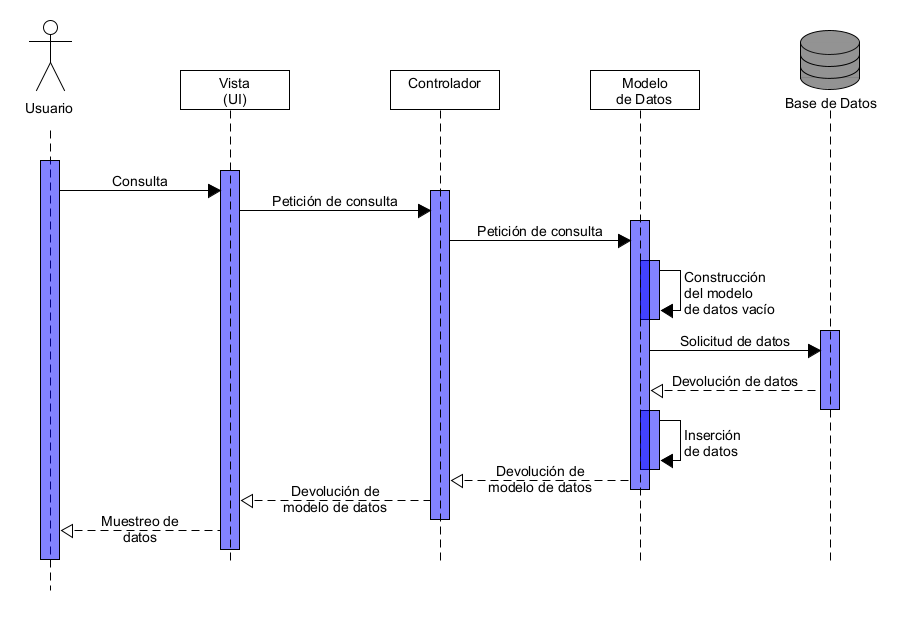
\includegraphics[width=\textwidth]{img/imgs-memoria/Secuencias_Consulta.png}
    \caption{Diagrama de secuencias de una consulta}
\end{figure}

El siguiente diagrama de secuencias representa la inserción o eliminación de datos por parte de un usuario, acciones también realizadas gracias a SQLAlchemy. En este tipo de acciones se encuentran la adición de alumnos, cursos y secciones por parte de un profesor, generación de calificaciones tras enviar una tarea por parte de un alumno y la emiminación de todos los tipos de datos anteriores:

\begin{figure}[H]
    \hspace*{-1.5cm} 
    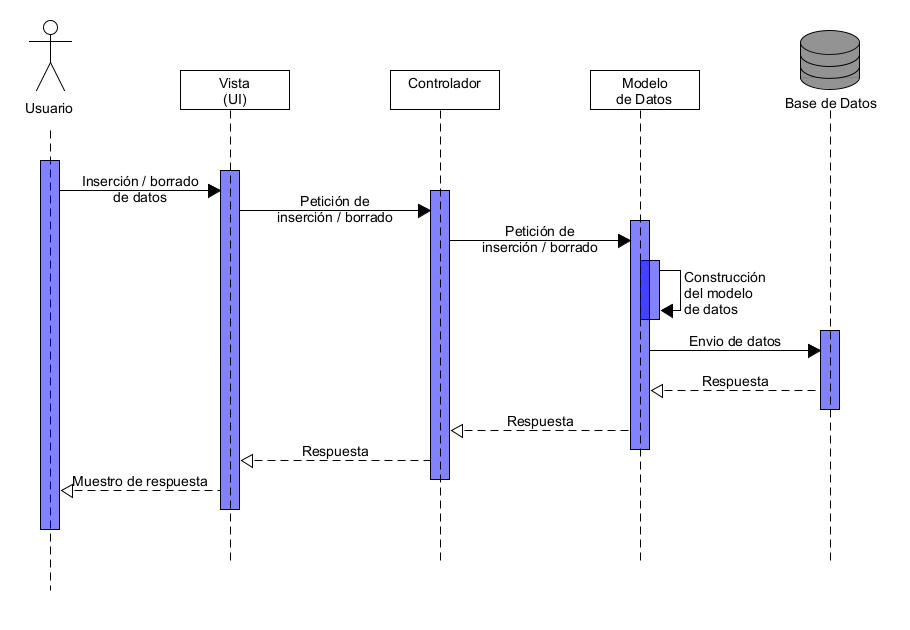
\includegraphics[scale=0.5]{img/imgs-memoria/Secuencias_Ins_DeL.png}
    \caption{Diagrama de secuencias de una inserción / borrado}
\end{figure}

Por último, en los siguientes diagramas se refleja el manejo de las acciones relacionadas con el autograding y generación de tareas mediante Nbgrader, acciones realizadas mediante la implementación de una clase de manejo (manager / gerente) de la API pública de esta herramienta:

\begin{figure}[H]
    \centering
    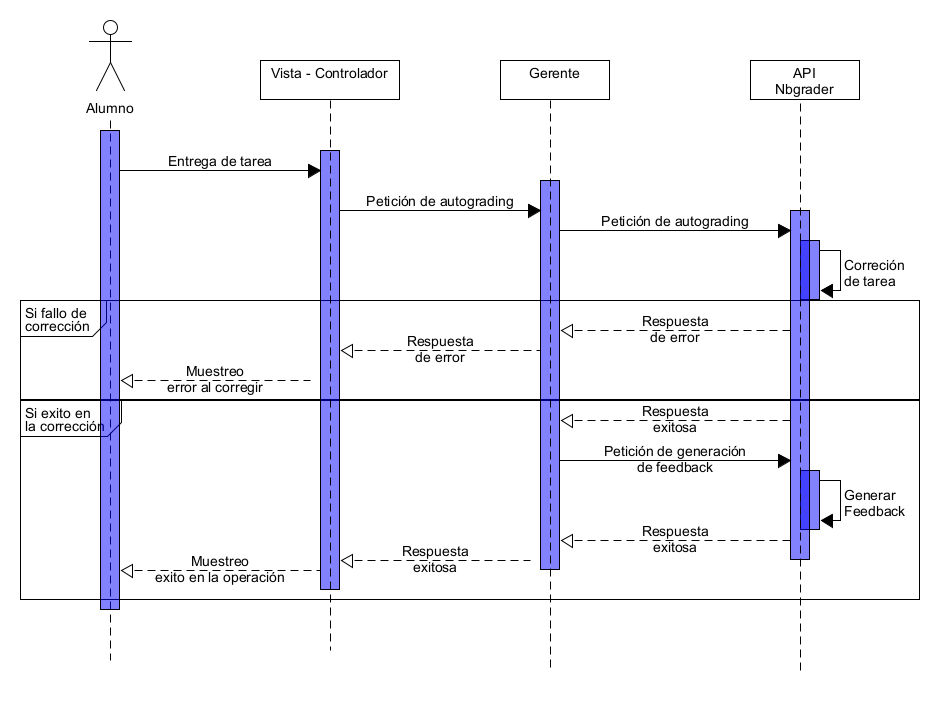
\includegraphics[width=\textwidth]{img/imgs-memoria/Secuencias_Autograding.png}
    \caption{Diagrama de secuencias autograding}
\end{figure}


\begin{figure}[H]
    \hspace*{-2cm} 
    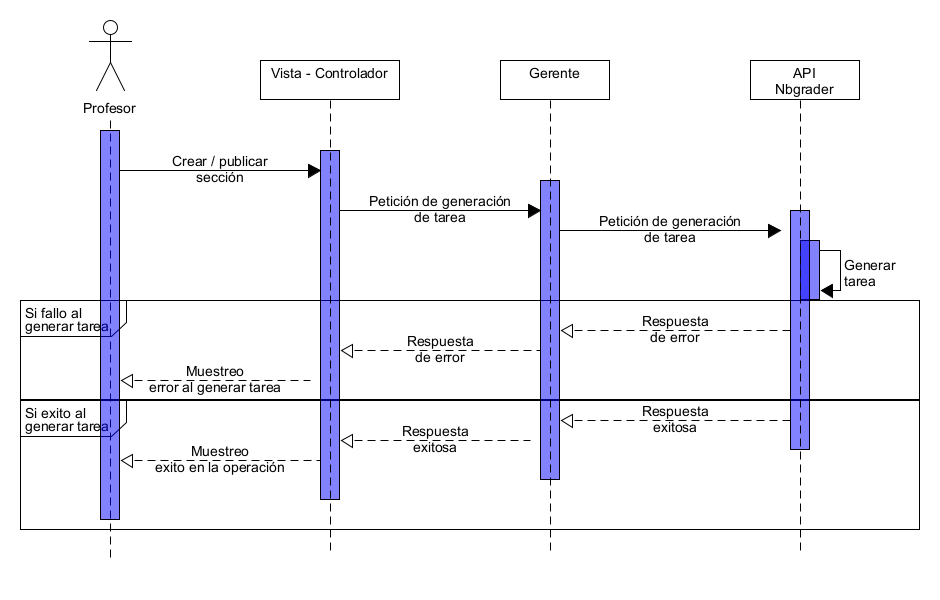
\includegraphics[scale=0.5]{img/imgs-memoria/Secuencias_Generate.png}
    \caption{Diagrama de secuencias generación de tarea}
\end{figure}


\section{Diseño arquitectónico}
Como ya se ha mencionado con anterioridad, el desarrollo de esta plataforma ha sido realizada mediante Flask. Flask es un framework minimalista no ligado a ningún diseño arquitectónico predefinido, lo cual ofrece a desarrolladores una gran libertad en cuanto a qué patrón arquitectónico dar a su proyecto.

En el caso de este proyecto, el patrón arquitectónico escogido ha sido \textbf{MVC (Modelo - Vista - Controlador)}:

\begin{figure}[H]
    \centering
    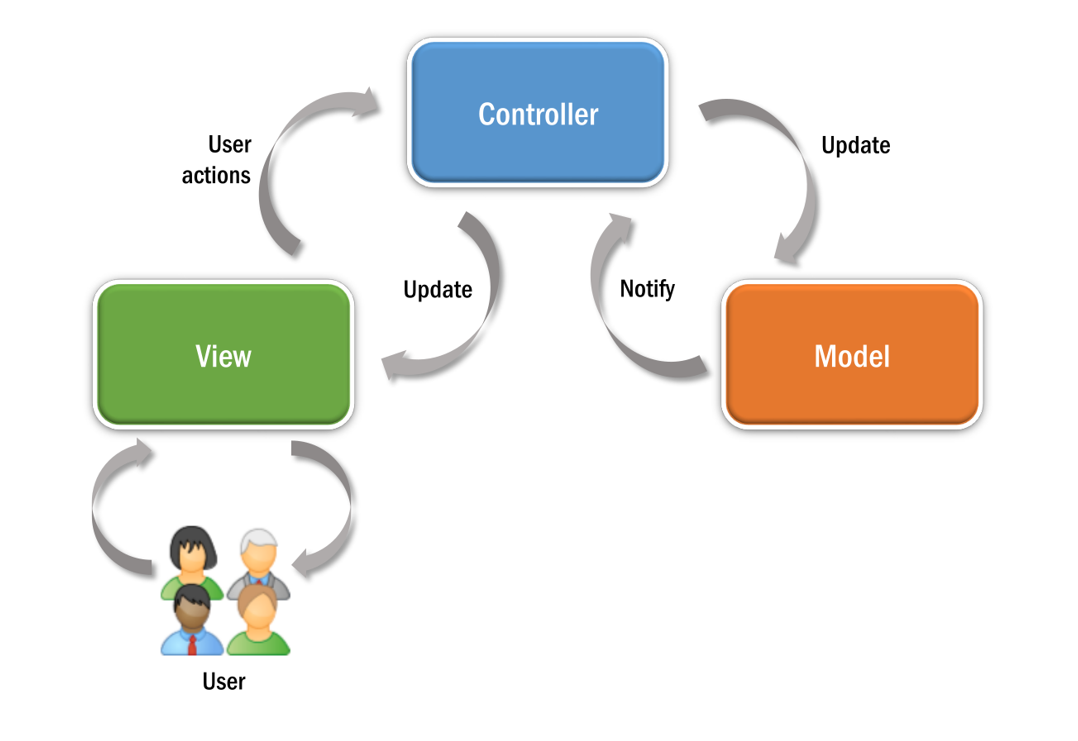
\includegraphics[scale=0.4]{img/imgs-memoria/MVC.png}
    \caption{Representación MVC}
\end{figure}

Este es un patrón software basado en la división de responsabilidades de una aplicación en tres capas diferentes:
\begin{itemize}
\item \textbf{Modelo:} Encargada de la representación y acceso a los datos del dominio junto con la lógica de negocio de estos.

\item \textbf{Vista:} Responsable de la generación de la interfaz de usuario, medio por el que los clientes visualizan la información e interactuan con el sistema.

\item \textbf{Controlador:} Intermediario entre las capas anteriores, encargado de gestionar el flujo de información entre las mismas.

\end{itemize}

En lo que a nuestro proyecto respecta, los métodos ruta o endpoints, que desempeñan la labor de Controlador, se encuentran en el fichero \textbf{routes.py}. La capa de Vista queda constituida por los directorios \textbf{templates} y \textbf{static} en los que se encuentran los documentos html, estilos e imágenes que componen la aplicación. La función de renderizado de vistas es desempeñada por el motor de templates Jinja2 sobre el que Flask está montado. Finalmente Flask no tiene predifinido ningún ORM (Asignación objeto-relacional) encargado de la función de Modelo y por ello la herramienta seleccionada para esta función es la mencionada con anteriordad SQLAlchemy.





\apendice{Documentación técnica de programación}

\section{Introducción}
El propósito de esta sección es la documentación de los componentes internos del proyecto y los aspectos más relevante de su desarrollo a nivel técnico, orientado a aquellas personas con conocimientos en informática interesadas en el desarrollo del mismo.

\section{Estructura de directorios}
El repositorio del proyecto, \textbf{accesible en la siguiente URL:} \url{https://github.com/AlbertoPorres/autograder-python}, cuenta con la siguiente estructura de directorios:
\begin{itemize}
\tightlist
\item \textbf{/:} Directorio raiz del proyecto. Contiene el fichero README y LICENSE para el proyecto, el archivo \textit{app.py} de ejecución de la aplicación, el archivo de requirements y Dockerfile para su instalación dentro de un contenedor Docker, el archivo de configuración de Jupyter Notebook y el resto de directorios del proyecto.
\item \textbf{/env:} Carpeta correspondiente a VirtualEnv donde se encuentran instaladas todas las dependencias de la aplicación para su correcta ejecución en el ambiente de desarrollo.
\item \textbf{/migrations:} Directorio de migraciones de la Base de Datos realizadas durante el desarrollo del proyecto.
\item \textbf{/src:} Directorio de código fuente del proyecto. En él se encuentra el archivo \textit{\_\_init\_\_.py} de configuración del proyecto flask, el archivo \textit{forms.py} correspondiente al manejo de formularios mediante Flask-Forms, el archivo \textit{management.py} correspondiente al manejo de la API de Nbgrader, el archivo \textit{models.py} correspondiente a los modelos de datos de SQLAlchemy, el archivo \textit{routes.py} donde se realizan las labores de controlador y la base de datos \textit{database.db} de la aplicación.
\item \textbf{/src/courses:} se encuentra el curso base que es utilizado como plantilla para la creación de nuevos cursos. En este directorio se almacenarán todos los cursos que se creen en la aplicación mediante el copiado y renombrado del curso base.
\item \textbf{/src/courses/base\_course:} curso base que contiene todos los directorios necesarios para el funcionamiento de Nbgrader (autograded, content, feedback, release, source y submitted), un notebook vacío utilizado para la creación de nuevas tareas dentro del curso mediante el copiado y renombrado del mismo, el archivo de configuración de Nbgrader \textit{nbgrader\_config.py}, la base de datos de Nbgrader \textit{gradebook.db} y un directorio adicional \textit{content} en el que se almacenan los archivos de contenido teórico de las secciones del curso.
\item \textbf{/src/static:} Contenidos estáticos de la aplicación. En él se encuentra el directorio de imégenes y el archivo \textit{base.css} de estilos.
\item \textbf{/src/static/imagenes:} Directorio de imágenes.
\item \textbf{/src/templates:} Directorio de archivos HTML.
\item \textbf{/doc:} Directorio documentación del proyecto.
\item \textbf{/doc/tex:} Directorio de archivos .text de la documentación.
\item \textbf{/doc/img:} Directorio de imágenes de la documentación.
\item \textbf{/Curso-Python:} Este directorio contiene los contenidos teóricos y tareas del curso de introducción a Python el cual ha sido añadido a la plataforma tras su despliegue vacío. Este contiene las 6 secciones de contenidos correspondientes a este curso (Introducción, Funciones, Listas y Tuplas, Control de Flujo, Diccionarios y Orientación a Objetos) divididas cada una en un directorio particular con su respectivo nombre. Dentro de cada directorio-sección se encuentran dos notebooks (archivos ipynb), el primero correspondiente al archivo de contenido teórico de la sección y cuyo nombre empieza por ''T\_'' (teoría) y el segundo correspondiente al archivo tarea en versión del profesor y cuyo nombre empieza por ''EV\_'' (evaluación).  

\end{itemize}

\section{Manual del programador}
Este manual tiene como objetivo dar información a futuros programadores que trabajen en el proyecto sobre los aspectos más importantes del código y herramientas de este.

\subsection{Prueba Nbgrader}
Tras considerar diversas herramientas de autocorrección de ejercicios \textit{Nbgrader} fue seleccionada como la herramienta de autograding a utilizar en nuestro proyecto. En esta sección queda documentada la primera toma de contacto con la herramienta en la que se realizó la instalación y prueba de esta. A diferencia de nuestro proyecto, en el cual las acciones de generación y corrección automática de tareas se realizan mediante el uso de la API pública de Nbgrader, en este primer manejo de la herramienta se hizo uso de la intefaz de usuario adicional que esta proporciona denominada Formgrader. Pese a ello, esta prueba demuestra la estructura de directorios de la que Nbgrader depende y nos proporciona nociones importantes sobre su funcionamiento:

\subsubsection{Instalación y preparación de ficheros}

Puesto que Nbgrader es un software de autocorreción de pruebas dependiente de Jupyter Notebook, el proceso de preparación de la herramienta para esta prueba fue el siguiente:

\begin{enumerate}
\item Instalación de la herramienta desde el terminal de Jupyter:

\begin{figure}[H]
    \centering
    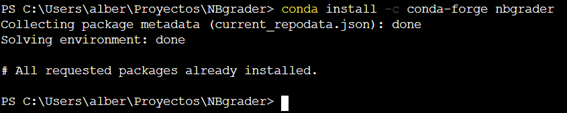
\includegraphics[width=0.8\textwidth]{img/instal/instal_1.png}
    \caption{Proceso de instalación 1}
\end{figure}

\item Debido a la forma en la que nbgrader busca las tareas y test y opera con ellos, se debe de crear una estructura concreta de ficheros en el directorio raíz. En primer lugar, se crea el fichero “submitted” (enviados) en el que se almacenarán las tareas enviadas por los alumnos:

\begin{figure}[H]
    \centering
    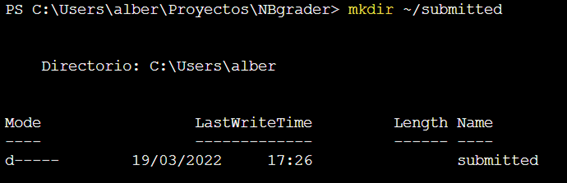
\includegraphics[width=0.8\textwidth]{img/instal/instal_2.png}
    \caption{Proceso de instalación 2}
\end{figure}

\item Dentro del directorio “submitted” se debe de incluir un fichero para las entregas de cada alumno, en este caso solo tendremos al alumno “alum1”:

\begin{figure}[H]
    \centering
    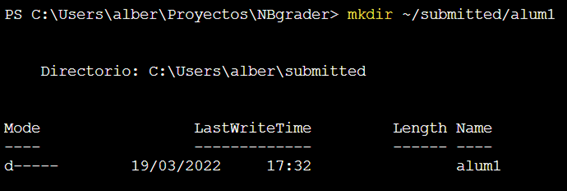
\includegraphics[width=0.8\textwidth]{img/instal/instal_3.png}
    \caption{Proceso de instalación 3}
\end{figure}

\item Dentro de los ficheros individuales de cada alumno se debe crear un fichero por cada tarea encargada, en este caso definimos una única tarea, “task1”:

\begin{figure}[H]
    \centering
    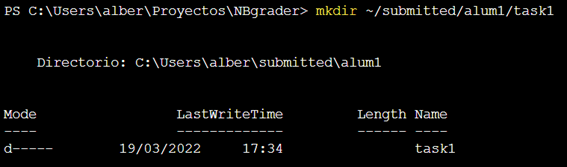
\includegraphics[width=0.8\textwidth]{img/instal/instal_4.png}
    \caption{Proceso de instalación 4}
\end{figure}

\item Los ficheros tareas enviadas por los alumno almacenadas en estas carpetas tendrán el mismo nombre que la carpeta de esa tarea correspondiente con una extensión .ipynb (notebook de jupyter).

\end{enumerate}


\subsubsection{Lanzamiento y creación de una tarea}

\begin{enumerate}
\item Una vez creada la estructura de ficheros reiniciamos jupyter notebook:	

\begin{figure}[H]
    \centering
    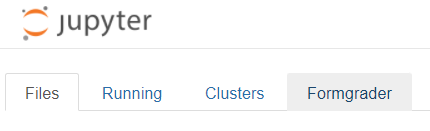
\includegraphics[width=0.8\textwidth]{img/prueba/prueba_1.png}
    \caption{Proceso de lanzamiento y creación 1}
\end{figure}

\item Al reiniciarlo nos habrá aparecido una nueva sección (Formgrader). En esta sección podremos gestionar la creación de tareas para los alumnos a través de la UI Formagrader:

\begin{figure}[H]
    \centering
    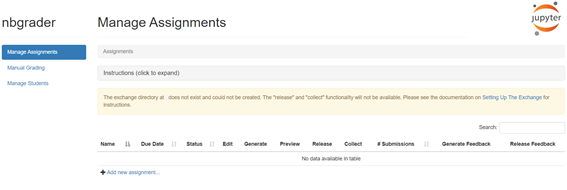
\includegraphics[width=0.8\textwidth]{img/prueba/prueba_2.png}
    \caption{Proceso de lanzamiento y creación 2}
\end{figure}

\item Para crear una nueva tarea, hacemos click en la opción “Add new assigment” y rellenamos los campos:

\begin{figure}[H]
    \centering
    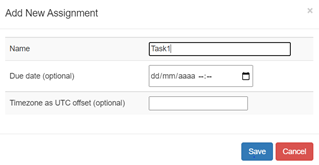
\includegraphics[width=0.8\textwidth]{img/prueba/prueba_3.png}
    \caption{Proceso de lanzamiento y creación 3}
\end{figure}

\begin{figure}[H]
    \centering
    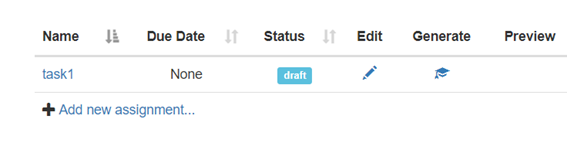
\includegraphics[width=0.8\textwidth]{img/prueba/prueba_4.png}
    \caption{Proceso de lanzamiento y creación 4}
\end{figure}

\item Para editar la tarea hacemos click en el nombre:

\begin{figure}[H]
    \centering
    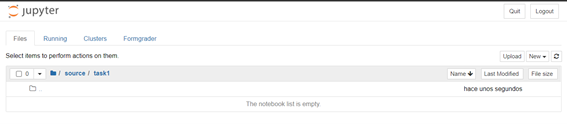
\includegraphics[width=1\textwidth]{img/prueba/prueba_5.png}
    \caption{Proceso de lanzamiento y creación 5}
\end{figure}

\item En esta sección creamos una nueva tarea (notebook) y editamos su nombre. Dentro del apartado de “view” (vista) podemos activar el modo de creación de tareas:

\begin{figure}[H]
    \centering
    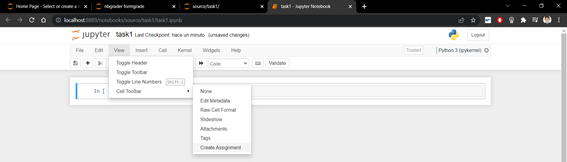
\includegraphics[width=1\textwidth]{img/prueba/prueba_6.png}
    \caption{Proceso de lanzamiento y creación 6}
\end{figure}

\item De esta manera las celdas tendrán diferentes formatos para la creación de la tarea:

\begin{figure}[H]
    \centering
    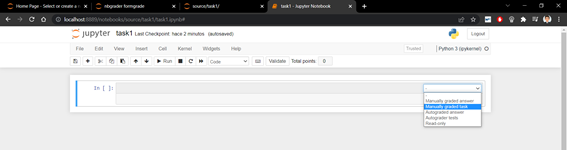
\includegraphics[width=1\textwidth]{img/prueba/prueba_7.png}
    \caption{Proceso de lanzamiento y creación 7}
\end{figure}

\item A continuación se puede crear nuestra primera prueba; se ha creado una prueba muy sencilla en la que se manda al alumno crear una función suma, para ello se crea una celda tipo “Autograded answer” en la que el profesor crea la función y deja entre los comentarios “\#\#\#BEGIN SOLUTION” y “\#\#\#END SOLUTION” la parte de código que el alumno ha de implementar. En la celda tipo “Autograded tests” se crean las pruebas para dicha función, estas pruebas están basadas es la ejecución de sentencias assert y se le ha de asignar una puntuación.

\begin{figure}[H]
    \centering
    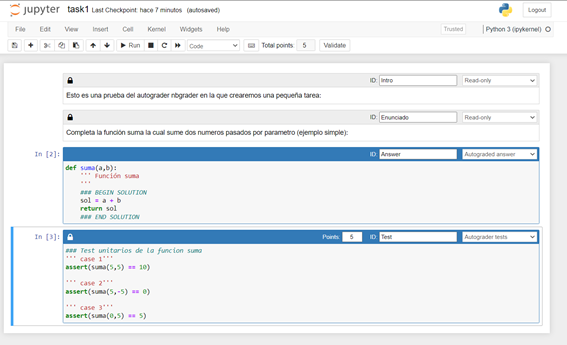
\includegraphics[width=1\textwidth]{img/prueba/prueba_8.png}
    \caption{Proceso de lanzamiento y creación 8}
\end{figure}

\item Una vez creadas las pruebas se ha de validar que el código del profesor es correcto y funciona por lo que se ha de hacer click en la casilla “validate” y en caso de que sea correcto recibiremos el siguiente mensaje:

\begin{figure}[H]
    \centering
    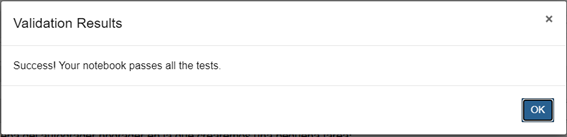
\includegraphics[width=1\textwidth]{img/prueba/prueba_9.png}
    \caption{Proceso de lanzamiento y creación 9}
\end{figure}

\item Una vez creado, volvemos a la sección de manejo de tareas:

\begin{figure}[H]
    \centering
    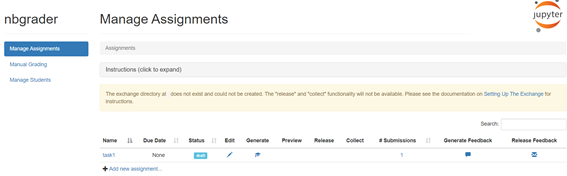
\includegraphics[width=1\textwidth]{img/prueba/prueba_10.png}
    \caption{Proceso de lanzamiento y creación 10}
\end{figure}

\item Para generar la tarea que sería entregada a los alumnos hacemos click en el icono de “generate” para la tarea correspondiente y recibiremos, en caso de funcionar correctamente, el siguiente mensaje:

\begin{figure}[H]
    \centering
    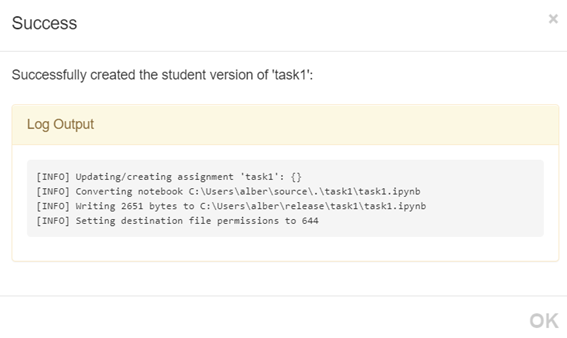
\includegraphics[width=1\textwidth]{img/prueba/prueba_11.png}
    \caption{Proceso de lanzamiento y creación 11}
\end{figure}

\item Una vez creado hacemos click en el apartado “preview” para previsualizarlo como un alumno lo vería:

\begin{figure}[H]
    \centering
    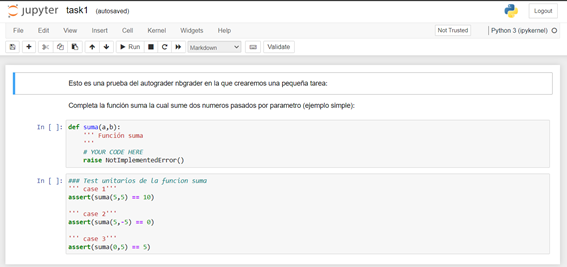
\includegraphics[width=1\textwidth]{img/prueba/prueba_12.png}
    \caption{Proceso de lanzamiento y creación 12}
\end{figure}

\item Como vemos en la casilla de la función suma, el contenido del código se ha modificado automáticamente para ser completado por el alumno.
Una vez hechos todos estos pasos ya tendríamos creada la tarea. En este momento nbgrader habrá generado automáticamente en el directorio raíz de tu equipo una nueva carpeta llamada “release” con la tarea correspondiente:

\begin{figure}[H]
    \centering
    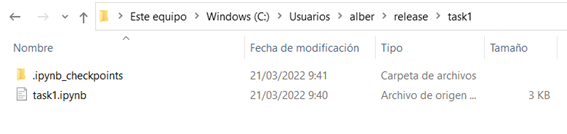
\includegraphics[width=1\textwidth]{img/prueba/prueba_13.png}
    \caption{Proceso de lanzamiento y creación 13}
\end{figure}

\item Este notebook será entregado al alumno para la realización de la tarea.

\end{enumerate}

\subsubsection{Realización de la tarea y corrección}

\begin{enumerate}
\item Una vez el alumno recibe la tarea y la completa: 

\begin{figure}[H]
    \centering
    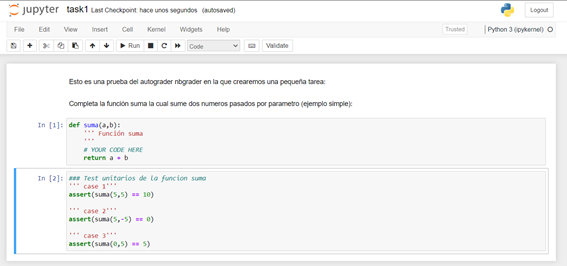
\includegraphics[width=1\textwidth]{img/prueba/prueba_14.png}
    \caption{Proceso de realización y corrección 1}
\end{figure}

\item Este puede comprobar su resultado haciendo click en el icono “validate” en caso de tener Nbgrader instalado:

\begin{figure}[H]
    \centering
    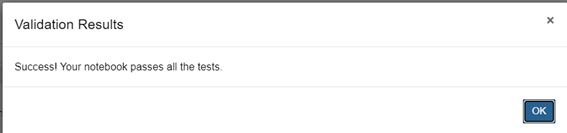
\includegraphics[width=0.8\textwidth]{img/prueba/prueba_15.png}
    \caption{Proceso de realización y corrección 2}
\end{figure}

\item Una vez haya acabado la tarea, la guardará y enviará de nuevo al profesor quien almacenará esta en el archivo dentro de submitted creado anteriormente para esa tarea:

\begin{figure}[H]
    \centering
    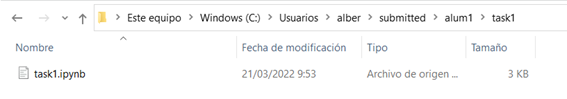
\includegraphics[width=1\textwidth]{img/prueba/prueba_16.png}
    \caption{Proceso de realización y corrección 3}
\end{figure}

\item Ahora el profesor accederá de nuevo al apartado de gestión de tareas:

\begin{figure}[H]
    \centering
    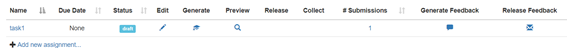
\includegraphics[width=1\textwidth]{img/prueba/prueba_17.png}
    \caption{Proceso de realización y corrección 4}
\end{figure}

\item Y accederá al apartado de submissions de la tarea:

\begin{figure}[H]
    \centering
    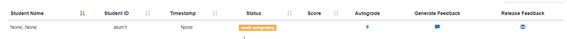
\includegraphics[width=1\textwidth]{img/prueba/prueba_18.png}
    \caption{Proceso de realización y corrección 5}
\end{figure}

\item Hacemos click en la opción “autograde”:

\begin{figure}[H]
    \centering
    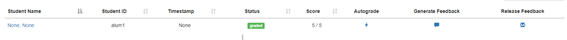
\includegraphics[width=1\textwidth]{img/prueba/prueba_19.png}
    \caption{Proceso de realización y corrección 6}
\end{figure}


\item Y como vemos se corrige automáticamente, en este caso el alumno ha aprobado. Adicionalmente si hacemos click en “generate feedback” nbgrader creará una carpeta “feedback” con documentos html con retroalimentación para el alumno:

\begin{figure}[H]
    \centering
    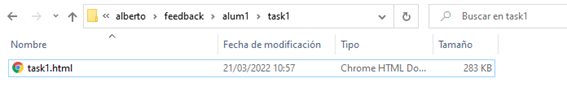
\includegraphics[width=1\textwidth]{img/prueba/prueba_20.png}
    \caption{Proceso de realización y corrección 7}
\end{figure}

\begin{figure}[H]
    \centering
    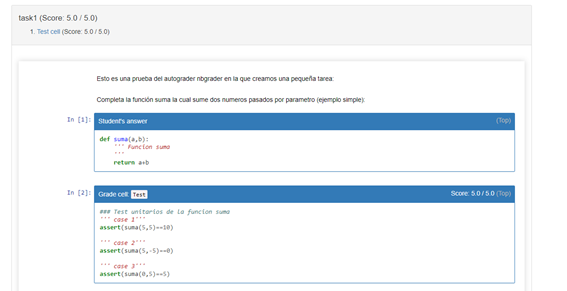
\includegraphics[width=1\textwidth]{img/prueba/prueba_21.png}
    \caption{Proceso de realización y corrección 8}
\end{figure}
\end{enumerate}

\subsection{Funcionamiento Nbgrader}
Como se ha visto en la prueba anterior, Nbgrader necesita una serie de directorios y archivos para su funcionamiento. La estructura de un curso sobre el que va a funcionar Nbgrader es la siguiente:
\begin{figure}[H]
    \centering
    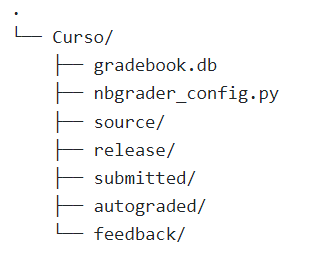
\includegraphics[scale=0.7]{img/imgs-memoria/NbgraderTree.PNG}
    \caption{Estructura Curso Nbgrader}
\end{figure}
\begin{itemize}
\item \textbf{gradebook.db:} Base de datos en la que Nbgrader almacena información sobre tareas, alumnos y entregas.
\item \textbf{nbgrader\_config.py:} Archivo de configuración de Nbgrader.
\item \textbf{source:} Directorio en el que se almacenan las tareas (notebooks) creadas por el profesor. Estos notebooks serán adaptados por Nbgrader para la generación de estos en versión alumno.
\item \textbf{release:} Directorio en el que se almacenan las tareas en versión del alumno tras ser generadas por Nbgrader.
\item \textbf{submitted:} Directorio en el que se almacenan las tareas entregadas por los alumnos.
\item \textbf{autograder:} Directorio en el que se almacenan las tareas corregidas.
\item \textbf{feedback:} Directorio en el que se almacenan los archivos feedback generados por Nbgrader de las tareas enviadas y corregidas.
\end{itemize}

En la siguiente tabla se muestran las diversas etapas en las que consiste el funcionamiento de Nbgrader con la información sobre los actores que realizan estas acciones, comandos utilizados, estructura de carpetas, archivos implicados y observaciones sobre estas:


\begin{landscape}
\begin{figure}[t]
    \hspace*{-2cm} 
    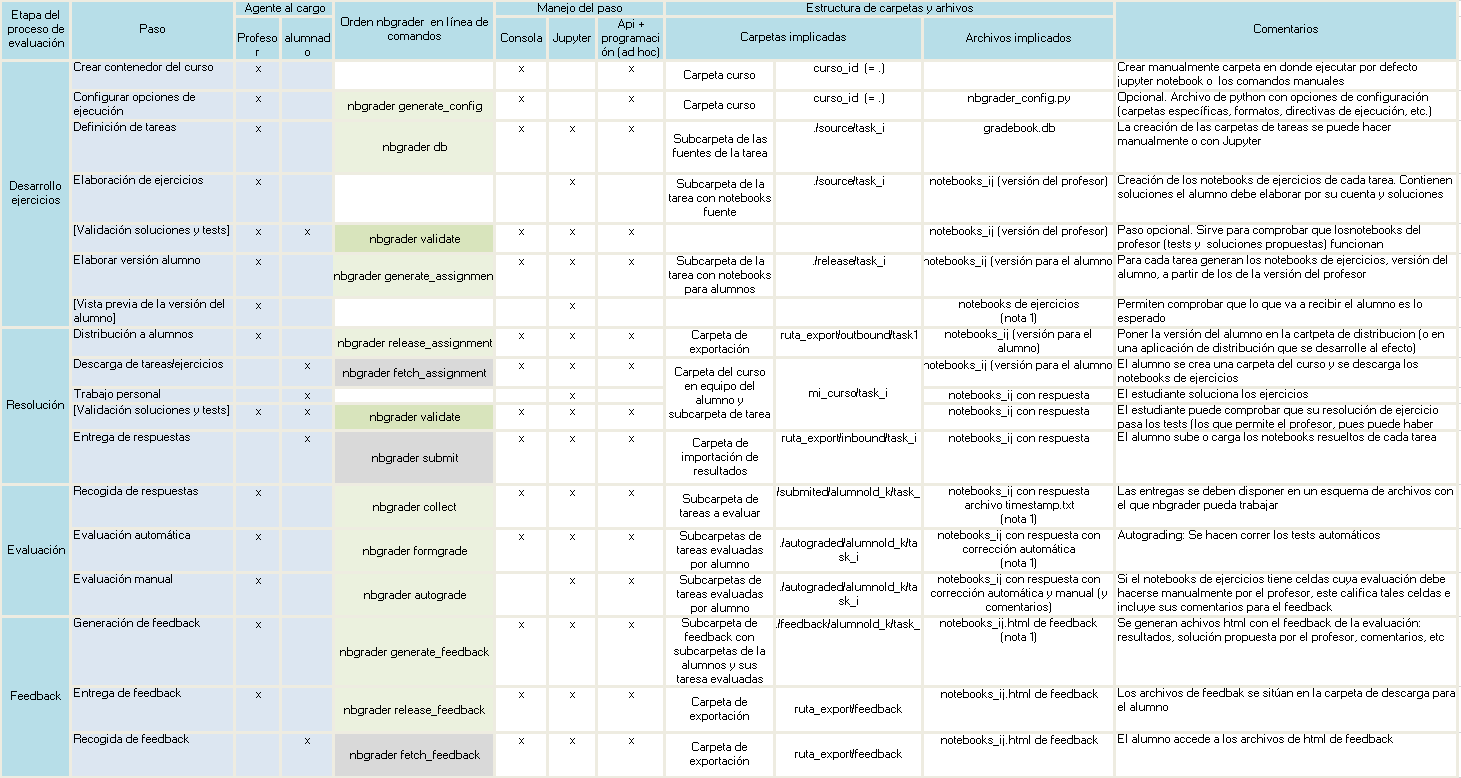
\includegraphics[scale=0.83]{img/imgs-memoria/Tabla_Nbgrader1.PNG}
    \caption{Tabla Nbgrader 1}
\end{figure}

\begin{figure}[t]
    \hspace*{-3cm} 
    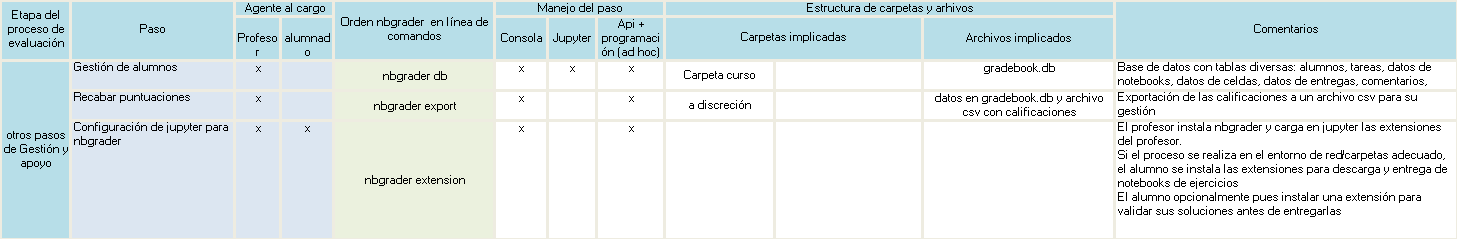
\includegraphics[scale=0.78]{img/imgs-memoria/Tabla_Nbgrader2.PNG}
    \caption{Tabla Nbgrader 2}
\end{figure}
\end{landscape}

\subsection{Creación de Cursos}
Ya se ha visto la estructura de archivos y directorios que necesita Nbgrader para su funcionamiento. Debido a esta dependencia estructural, la forma en la que ha sido implementada la creación de cursos dentro del proyecto ha consistido en el copiado y renombrado del directorio de un curso base el cual contiene todos los archivos y directorios necesarios para el funcionamiento de Nbgrader y la creación de tareas. Este curso se encuentra dentro de la carpeta \textit{courses} que es la propia carpeta en la que el resto de cursos serán añadidos:

\begin{figure}[H]
    \centering
    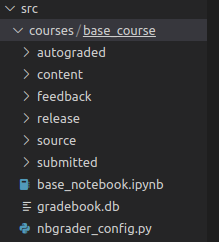
\includegraphics[scale=1]{img/imgs-memoria/base_course.PNG}
    \caption{Curso base}
\end{figure}

Adicionalmente, este curso base contiene el directorio \textit{content} cuya función es el almacenamiento de los archivos teóricos pertenecientes al curso.

El endpoint o método-ruta en el que es realizada esta acción es el denominado \textbf{teacher\_create\_course()} y concretamente la sección de código en la que se realiza esta acción es la siguiente:

\begin{figure}[H]
    \centering
    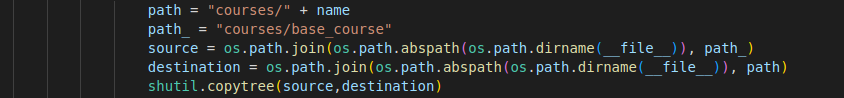
\includegraphics[scale=0.8]{img/imgs-memoria/Code_createCourse.PNG}
    \caption{Código creación curso}
\end{figure}


\subsection{Manejo de Nbgrader}
El manejo de Nbgrader dentro del proyecto se realiza mediante la clase \textbf{NbgraderManager} dentro del módulo \textbf{Management.py}.

\subsubsection{Construcción}
El constructor de esta clase es el siguiente:

\begin{figure}[H]
    \centering
    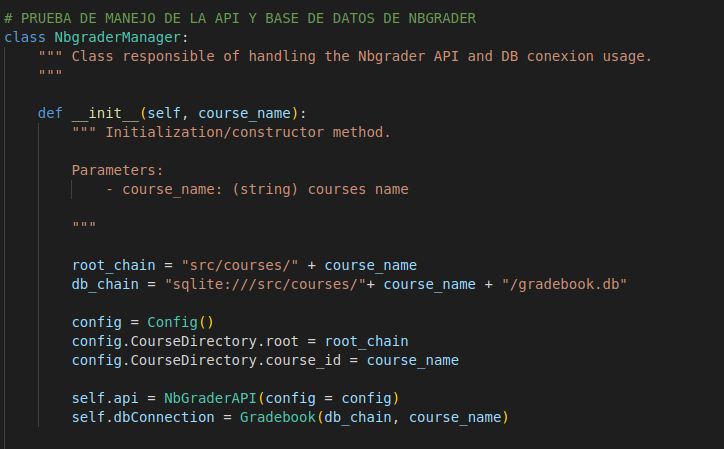
\includegraphics[scale=0.8]{img/imgs-memoria/ConstructorManager.PNG}
    \caption{Constructor manager}
\end{figure}

En este se está estableciendo la conexión con la base de datos \textit{gradebook.db} de Nbgrader dentro de la carpeta del curso pasado por parámetro sobre el que se van a realizar las acciones de Nbgrader. Adicionalmente se crea la variable de instancia de la API de Nbgrader por la que se ejecutarán las funciones de este. 

\subsubsection{Acciones más importantes}
Las operaciones más importantes del manager son las siguientes:

\begin{itemize}
\item \textbf{Grade:} Manda a la API de Nbgrader la realización de la corrección de una tarea accediendo a esta en la carpeta submitted del alumno pasado por parámetro y, en caso de tener éxito en la operación, accede a la base de datos para obtener la calificación obtenida, redondeándola sobre 10:
\begin{figure}[H]
    \centering
    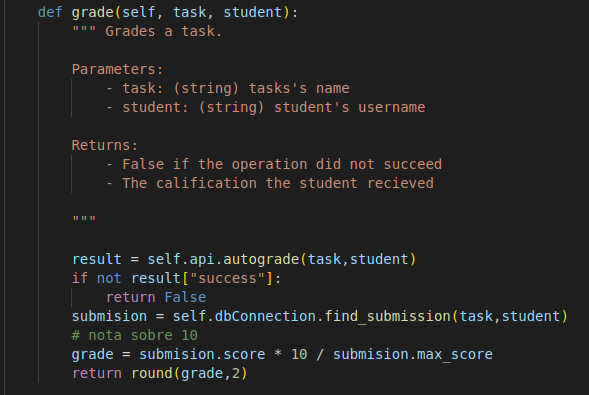
\includegraphics[scale=0.8]{img/imgs-memoria/Grade.PNG}
    \caption{Corrección de tarea}
\end{figure}

Este método es llamado desde el endpoint \textbf{student\_course()} al realizarse la entrega de una tarea por parte de un alumno.

\item \textbf{Create assigment:} Manda a la API de Nbgrader la generación de una tarea en versión de estudiantes. Para ello, accede a la tarea dentro de la carpeta source del curso:
\begin{figure}[H]
    \centering
    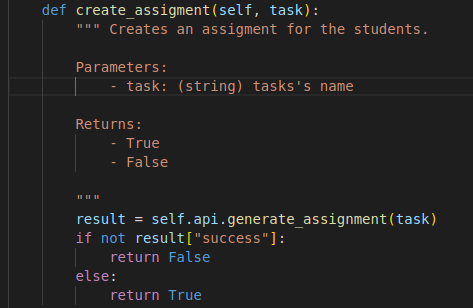
\includegraphics[scale=0.8]{img/imgs-memoria/CrearTarea.PNG}
    \caption{Generación de tarea para los alumnos}
\end{figure}

Este método es llamado cuando un profesor crea una sección de contenido de forma directa en la que entrega el notebook tarea creado previamente, acción realizada en el endpoint \textbf{teacher\_create\_section(course)}. O cuando el profesor ordena la publicación de una sección de contenido no publicada, acción realizada en el endpoint \textbf{publish\_section(course,section)}.

\item \textbf{Generate feedback:} Manda a la API de Nbgrader la generación del documento feedback de una tarea entregada por un alumno:

\begin{figure}[H]
    \centering
    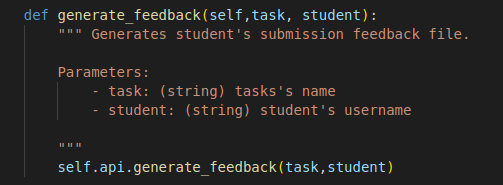
\includegraphics[scale=0.8]{img/imgs-memoria/generateFeedback.PNG}
    \caption{Generación de feedback}
\end{figure}

Este método es llamado tras la correcta corrección automática de una tarea al ser entregada por un alumno en el endpoint \textbf{student\_course()}.

\end{itemize}

\subsection{Creación de tareas desde la plataforma}

Ya ha sido mencionado con anterioridad el hecho de que una de las funcionalidades de la plataforma consistía en permitir a los profesores la creación de tareas desde la propia plataforma. Para lograr esto fueron añadidas las denominadas \textbf{Secciones no publicadas}. Estas secciones son creadas por el profesor dentro de uno de sus cursos y son solo visualizables por él y no por los alumnos, hasta su publicación o descarte. Al crearse una sección no publicada por un profesor, este define el nombre que tendrá el notebook tarea la cual es incluida en la carpeta \textit{source} del curso. Posteriormente, el profesor puede ver el listado de las secciones no publicadas del curso y acceder a la tarea que desee editar, momento en el que se le abrirá en su navegador una nueva pestaña en la que se está accediendo, mediante la ejecución remota de Jupyter Notebook, al notebook específico. Para lograr esto, Jupyter Notebook junto con Nbgrader se encuentra instalado dentro del propio proyecto y es ejecutado remótamente desde el momento inicial en el que la app es iniciada. Los comandos para lograr esto son los siguientes:

\begin{figure}[H]
    \centering
    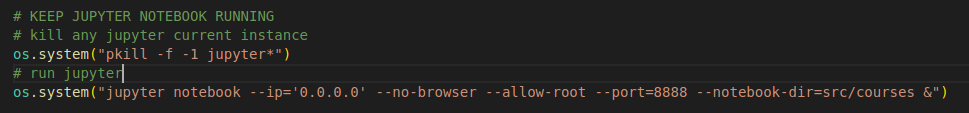
\includegraphics[scale=0.8]{img/imgs-memoria/RunJupyter.PNG}
    \caption{Ejecución de Jupyter}
\end{figure}

Para lograr la apertura del notebook tarea concreto que el profesor desea editar, se incluye la siguiente línea de código dentro del template de vistas de secciones sin publicar \textbf{unreleased\_sections.html}: 

\begin{figure}[H]
    \hspace*{-1.5cm} 
    \includegraphics[scale=0.8]{img/imgs-memoria/AbrirNotebook.PNG}
    \caption{Apertura Notebook}
\end{figure}

Esta se encarga de abrir en una nueva pestaña el notebook específico, introduciendo la URL de este. Para ello se ha tenido que introducir la IP específica de la ruta de ejecución remota de nuestro Jupyter Notebook (la cual ha sido ocultada en esta imagen por seguridad), por ello, se debía conocer con anterioridad la IP sobre la que nuestra plataforma ha sido desplegada.

Cuando un profesor decide publicar una sección no publicada, la orden de generación de tarea es llamada, cogiendo el archivo correspondiente a esa sección en el fichero \textit{source} y generando dentro de \textit{release} la versión correspondiente a los alumnos. 


\subsubsection{Librerías y métodos relevantes utilizados}
En esta sección van a ser descritas algunas de las librerías y métodos más relevantes utilizados en el proyecto junto con su utilidad dentro del mismo:
\begin{itemize}
\item \textbf{os:} El módulo de Python os permite el uso de funcionalidades de sistema operativo de forma versatil. En nuestro proyecto, los métodos y módulos derivados de este utilizados han sido:
    \begin{itemize}
        \item \textbf{system:} Ejecución de comandos de sistema operativo. Ha sido utilizado para el lanzamiento de Jupyter Notebook desde el proyecto.
        \item \textbf{remove:} Método de borrado de ficheros dentro de un directorio. Ha sido utilizado para el borrado de envíos, borrado de archivos de contenido teórico y tareas dentro de los directorios \textit{source} de los cursos en la cancelación de secciones, borrado de archivos de contenido teórico en la eliminación de secciones y borrado de tareas en la entrega de las mismas por los alumnos en caso de no haberse podido realizar el autograding por problemas en ella.
        \item \textbf{path:} Modulo de manejo de rutas de archivos y directorios.
        \item \textbf{mkdir:} Método de creación de directorios. Ha sido utilizado para la creación de directorios fundamentales para el funcionamiento de Nbgrader.
        \item \textbf{rename:} Método de renombrado de archivos. Ha sido utilizado para el renombre de archivos en la creación de tareas de secciones no publicadas, tras realizarse la copia del notebook base encontrado en cada curso.
    \end{itemize}
\item \textbf{shutil:} El módulo de Python shutil permite realizar Operaciones de archivos de alto nivel. En nuestro proyecto, los métodos y módulos derivados de este utilizados han sido:
    \begin{itemize}
        \item \textbf{rmtree:} Método de borrado de rutas de directorios. Ha sido utilizado para el borrado de carpetas de alumnos dentro de los directorios \textit{feedback} y \textit{submitted} en el borrado de alumnos o extracción de los mismos de un curso, borrado de directorios que habían sido creados con anterioridad en la creación de secciones que han dado error de generación de tarea, cancelación de secciones no publicadas, borrado de cursos, eliminación de secciones y actividades similares.
        \item \textbf{copytree:} Método de copiado de árboles de archivos. Ha sido utilizado en la creación de nuevos cursos.
        \item \textbf{copy:} Método de copiado de archivos. Ha sido utilizado en la creación de nuevas tareas.
    \end{itemize}
\item \textbf{flask.send\_from\_directory():} Método de Flask para el envío de ficheros de un directorio. Utilizado para la descarga de archivos por parte de los usuarios.
\end{itemize}

\subsection{Montaje en Docker}

El Dockerfile a partir del que se ha generado la imagen del contenedor en el que ha sido instalada nuestra plataforma es el siguiente:


\begin{figure}[H]
    \centering
    \includegraphics[scale=0.9]{img/imgs-memoria/Dockerfile.PNG}
    \caption{Dockerfile}
\end{figure}

En este se está ordenando la copia del proyecto junto con la instalación de todas sus dependencias software para su correcto funcionamiento. Adicionalmente, es introducida en la ruta de configuración de Jupyter Notebook el fichero \textbf{jupyter\_notebook\_config.py} el cual ha sido modificado deshabilitando la apertura de terminales y el botón de parada del kernel de ejecución para, en caso de que un profesor intente pararlo, este no pueda ya que esto generaría un problema en la edición de tareas desde la plataforma.

Una vez creada la imagen del contenedor a partir del dockerfile mediante la ejecución del comando \textbf{docker build -t "nombre\_imagen" .}.Este ha de ser ejecutado realizando el mapeo de puertos adecuado. Nuestra aplicación flask es lanzada a través del puerto local 5000 y Jupyter Notebook es ejecutado a través del 8888, por ello, el comando de construcción del contenedor con el mapeo de puertos correcto sería: \textbf{docker run -d -t --name=*nombre* -p *puerto de salida deseado para flask*:5000 -p *puerto de salida deseado para Jupyter*:8888 *nombre\_imagen*}. Una vez esté corriendo el contenedor con el mapeo de puertos correcto, se ha de acceder a este mediante el comando: \textbf{docker exec -ti *nombre* bash}.


Al ser ejecutado Jupyter de forma remota y accedido en un navegador web por primera vez, Jupyter pide al usuario que introduzca un token que este genera de forma automática, o una contraseña previamente establecida como forma de seguridad ante el intento de acceso a usuarios no autorizados. Puesto que los profesores que accedan de forma remota a Jupyter no tendrán acceso a este token generado automáticamente dentro del contenedor Docker, se ha de establecer una contraseña previa al lanzamiento de la aplicación. Para ello, una vez instalado el proyecto dentro del correspondiente contenedor Docker, se ha de establecer una contraseña mediante el comando \textbf{jupyter notebook password}. En el caso de nuestra plataforma, la contraseña que los profesores tendrán que introducir la primera vez que accedan a jupyter al crear o editar una tarea de forma remota será la palabra "teacher".

Una vez realizado el paso previo nuestra aplicación estaría lista para su ejecución desde el contenedor, acción que es realizada mediante la ejecución del comando \textbf{python3 app.py}. Tras esto nuestra aplicación podrá ser accesible de forma local en un navegador en la dirección \textbf{http://localhost:5000}.


\subsection{Riesgo de la ejecución remota de Jupyter Notebook}
El hecho de estar ejecutando jupyter notebook de forma remota con el fin de hacer posible la edición de tareas supone un inconveniente de seguridad. Este inconveniente consiste en que en el momento en el que un profesor está editando una tarea, este puede retroceder en el árbol de archivos de jupyter notebook, viendo así carpetas correspondientes al funcionamiento interno de los cursos:

\begin{figure}[H]
    \centering
    \includegraphics[width=14cm]{img/imgs-memoria/EdicionTarea.PNG}
    \caption{Edición de tarea}
\end{figure}

\begin{figure}[H]
    \centering
    \includegraphics[width=14cm]{img/imgs-memoria/arbol archivos.PNG}
    \caption{Acceso carpetas de cursos}
\end{figure}

Como se puede ver en las imágenes anteriores, el profesor ha pasado de editar una tarea a ver las carpetas de los cursos de la página retrocediendo en la ruta de archivos de Jupyter. Este incoveniente de seguridad no es especialmente preocupante al ser los propios profesores quienes pueden acceder a estos archivos, pero es la principal razón por la que no se permite a los alumnos contestar a las tareas desde la propia web, sino que han de resoverlas de forma local habiéndose descargado la tarea. Si un alumno pudiera realizar esta acción, tendría acceso a todos los contenidos de los cursos incluidas las versiones de las tareas del profesor, lo que podría dar lugar a la realización de trampas para superar las tareas o incluso problemas de funcionamiento de la plataforma en el caso de que estos decidieran eliminar algún directorio o archivo. La resolución de este problema ha sido propuesta como una posible futura línea de trabajo en el apartado de conclusiones y futuras líneas de trabajo de la memoria.

\section{Instalación, ejecución y despliegue del proyecto}

\subsection{Instalación}
Puesto que se ha hecho uso de la herramienta VirtualEnv la instalación de nuestro proyecto \textbf{en un ambiente de desarrollo Ubuntu / Linux} es una tarea muy sencilla. Para ello simplemente se ha de clonar el repositorio del mismo el cual tiene incluida la carpeta env correspondiente a esta herramienta.

\subsection{Ejecución desde el entorno de desarrollo}

Para la ejecución de nuestra aplicación de forma local en el ambiente de desarrollo se ha de activar el ambiente virtual mediante el comando \textbf{source env/bin/activate} desde el directorio raíz del proyecto. Una vez hecho esto, nuestra aplicación puede ser lanzada mediante el comando \textbf{python3 app.py}.

Adicionalmente, puesto que el estado final en el que se encuentra el proyecto dentro del repositorio está pensado para el despliegue directo de la plataforma, se puede activar dentro del archivo de lanzamiento \textbf{app.py} el modo de depuración, asignando el valor ''True'' al parámetro ''Debug'' del método de ejecución Flask de la aplicación:

\begin{figure}[H]
    \centering
    \includegraphics[scale=0.9]{img/imgs-memoria/DebugOn.PNG}
    \caption{Modo de depuración}
\end{figure}

\subsection{Despliegue}
La plataforma ha sido desplegada en una instancia EC2 de Amazon Web Service. En este apartado se va a explicar el proceso seguido para lograrlo en caso de que futuros programadores quieren realizar el mismo tipo de despliegue:

\begin{itemize}
\item Creación de la instancia t2.micro con imagen Amazon Linux gratuita de arquitectura 64 bits, par de claves RSA y formato de archivo pem y permitiendo el trafico HTTP desde internet.

\item Acceso a la instancia como cliente SSH. 

Comando: \textbf{ssh -i *Tu\_Archivo\_Clave.pem* ec2-user@ec2-3-89-140-10.compute-1.amazonaws.com}

\item Instalación de Docker y Git dentro de la instancia. Comandos: \textbf{sudo amazon-linux-extras install docker} y \textbf{sudo yum install Git}

\item Clonación del repositorio. Comando \textbf{Git clone *url*}

\item Asignación de permiso al usuario ec-2. Comando \textbf{sudo usermod -a -G docker ec2-user}.

\item Salida y vuelta a entrar a la instancia para la correcta asignación de permisos.

\item Creación de la imagen mediante docker build.

\item Lanzamiento del contenedor dentro de la instancia con el mapeo correcto de puertos. El puerto de salida de la plataforma Flask sobre el que se accederá a esta queda a elección del programador, en nuestro caso ha sido seleccionado el puerto 80. El puerto de salida de Jupyter Notebook ha de ser el 8888 por obligación ya que es hacia el que la plataforma redirecciona al abrir las tareas. 

\item Acceso al contenedor, establecimiento de la contraseña de Jupyter Notebook y lanzamiento de la aplicación como ha sido descrito en el apartado de Montaje en Docker del Manual del programador.

\item Adición de las dos reglas de entrada correspondientes a los dos puertos de nuestra plataforma dentro del grupo de seguridad de la instancia EC2. Tipo de reglas TCP personalizado y puertos 8888 (Jupyter Notebook) y el asignado a la salida de la aplicación Flask.

\item Salida de la instancia.
\end{itemize}

Una vez realizados los siguientes pasos nuestra plataforma será accesible en la url: \textbf{http://*IP\_INSTANCIA*:80}.
\apendice{Documentación de usuario}

\section{Introducción}
Esta apendice contiene la información orientada a los usuarios, tanto profesores como alumnos, para el correcto acceso y manejo de la plataforma.

\section{Requisitos de usuarios}

\subsection{Requisitos de profesores}
Para poder dar un uso adecuado a la aplicación se recomienda a los profesores la instalación de \textbf{Jupyter Notebooks} y \textbf{Nbgrader} en su entorno de trabajo personal para la creación de tareas. Estos pueden prescindir de ello ya que la plataforma permite edición de tareas desde esta pero, en el caso de que requieran visualizar las entregas de los alumnos descargadas, necesitaran de al menos \textbf{Jupyter Notebooks} para hacerlo.

En cuanto al acceso a la plataforma no se requiere de ningún requisito previo debido a la naturaleza web de esta. Estos podrán acceder a ella en el siguiente enlace \url{http://3.89.140.10/}.

\subsection{Requisitos de alumnos}
En lo que a los alumnos respecta, estos deberán tener instalado de forma obligatoria \textbf{Jupyter Notebooks} en su entorno de trabajo para la resolución de tareas.

Como se ha mencionado previamente, no se requiere de ningún requisito previo en cuanto al acceso a la plataforma web. Estos podrán acceder a ella en el siguiente enlace \url{http://3.89.140.10/}.

\section{Instalación}
Al tratarse de una plataforma web no es necesaria ninguna instalción previa para el acceso a esta. Alumnos y profesores podrán acceder a la plataforma en el siguiente enlace: \url{http://3.89.140.10/}.



\section{Manual del profesor}
A continuación se explicará el manejo de la plataforma orientado a los profesores:

\subsection{1 Acceso a la Plataforma}
El acceso a la plataforma es realizado a través del siguiente enlace: \url{http://3.89.140.10/} el cual nos lleva a la página inicial de esta.

\begin{figure}[H]
    \centering
    \includegraphics[width=\textwidth]{img/imgs-memoria/Landing.PNG}
    \caption{Página Inicial}
\end{figure}

\subsection{2 Inicio de Sesión}
El proceso de inicio de sesión contiene los siguientes paso:
\begin{itemize}
\tightlist
    \item Una vez accedido a la Página incial hacer click en el botón \textbf{Acceder} lo cual nos llevará a la página de inicio de sesión:
        \begin{figure}[H]
        \centering
        \includegraphics[width=\textwidth]{img/imgs-memoria/InicioSesion.PNG}
        \caption{Pagina Inicio de sesión}
        \end{figure}
    \item Introducir los credenciales de inicio de sesión y hacer click en el botón \textbf{Login}. Han sido incluido en el fichero README del repositorio los credenciales de acceso de los 5 profesores definidos incialmente para la aplicación.
    \item Si los credenciales son correctos será llevado a la página principal del profesor:
        \begin{figure}[H]
        \centering
        \includegraphics[width=\textwidth]{img/imgs-memoria/TeacherMain.PNG}
        \caption{Página Principal Profesor}
        \label{PagProfesor}
        \end{figure}
\end{itemize}


\subsection{3 Gestión de Cursos}
Para ir a la página de gestión de cursos del profesor se ha de hacer click en el botón \textbf{Ir a mis Cursos} de la \textbf{Página Principal del Profesor}(\ref{PagProfesor}) o en el botón \textbf{Cursos} de la barra navegacional superior. Esto nos llevaría a la página de gestión de cursos en la que se encuentran todos los cursos creados por este profesor:
\begin{figure}[H]
\centering
\includegraphics[width=\textwidth]{img/imgs-memoria/PaginaCursosProfesor.PNG}
\caption{Página de Cursos Profesor}
\label{PagCursosProfesor}
\end{figure}

\subsubsection{3.1 Creación de cursos}
Para la creación de un nuevo curso:
\begin{itemize}
\tightlist
\item Hacer click en el botón \textbf{Crear curso} de la \textbf{Página de Cursos del Profesor}(\ref{PagCursosProfesor}) lo cual le llevará al formulario de creación de un nuevo curso:
\begin{figure}[H]
\centering
\includegraphics[width=\textwidth]{img/imgs-memoria/CrearCurso.PNG}
\caption{Página de Creación de Curso}
\end{figure}
\item Introducción de los datos (nombre y descripción) del curso a crear.
\item Hacer click en el botón \textbf{Crear}.
\item Hacer click en el botón \textbf{Confirmar} del modal de confirmación desplegado.
\item Si los datos no pertenecen a otro curso su curso será creado y visualizable desde la \ref{PagCursosProfesor} \textbf{Página de Cursos del Profesor}.
\end{itemize}


\subsubsection{3.2 Borrado de cursos}
Para el borrado de cursos se ha de hacer click en el botón \textbf{Eliminar} del curso deseado desde la \textbf{Página de Cursos}(\ref{PagCursosProfesor}), esto desplegará un modal de confirmación de acción que borrará el curso al hacer click en \textbf{Confirmar}.




\subsubsection{3.3 Gestión de alumnos de un curso}
El proceso de gestión de alumnos de un curso, que permite el ingreso o expulsión de alumnos a un curso, se realiza de la siguiente manera:
\begin{itemize}
\tightlist
\item Hacer click en el botón \textbf{Gestión de estudiantes} del curso deseado desde la \textbf{Página de Cursos}(\ref{PagCursosProfesor}). Esto nos llevará a la página de gestión de alumnos del curso:
\begin{figure}[H]
\centering
\includegraphics[width=\textwidth]{img/imgs-memoria/GestionAluCurso.PNG}
\caption{Página de Gestión de Alumnos de un Curso}
\end{figure}
\item Mediante los botones de \textbf{Sacar del curso} y \textbf{Ingresar en el curso} podrá expulsar alumnos matriculados o ingresar alumnos no matriculados al curso. La confirmación de estas acciones se hace haciendo click en el botón \textbf{Confirmar} del modal desplegado al hacer click en los botones anteriores.
\end{itemize}


\subsubsection{3.4 Acceso y gestión de contenidos de un curso}
Para ir a la página de un curso en particular, desde la que se puede realizar la gestión de su contenido, se ha de hacer click en el botón \textbf{Acceder} del curso en la \textbf{Página de Cursos del Profesor}(\ref{PagCursosProfesor}). La página/vista de un curso particular es la siguiente:
\begin{figure}[H]
\centering
\includegraphics[width=\textwidth]{img/imgs-memoria/CursoIndividual.PNG}
\caption{Página de Gestión de Contenidos de un curso}
\label{PagContProf}
\end{figure}
Los cursos se organizan en \textbf{secciones de contenido}cada una de las cuales está \textbf{constituida por un documento teórico} cuyo formato queda a elección del profesor (PDF, DOCX, IPYNB, ...) \textbf{y una tarea corregible automáticamente en su entrega} en formato IPYNB creada mediante Jupyter Notebook y Nbgrader por el profesor. 


Desde esta vista podrá:
\begin{itemize}
\tightlist
\item Descargar contenidos teóricos, tareas en versión profesor y tareas en versión alumno a través de los botones \textbf{Descargar contenido teórico, Descargar tarea versión profesor y Descargar tarea versión alumnos} de cada sección de contenido actual del curso.
\item Eliminar secciones actuales del curso mediante el botón \textbf{Eliminar} de cada una de ellas.
\item Ir a la creación de sección de forma directa, creación de sección no publicada o gestión de las mismas (estos procesos serán descritos a continuación).
\end{itemize}

\subsubsection{3.4.1 Creación de sección de forma directa}
Para crear una sección de contenido de forma directa se ha de hacer click en el botón \textbf{Crear sección} de la \textbf{Página de gestión de contenidos de un curso}(\ref{PagContProf}) en particular, lo que nos lleva al formulario de creación de sección:

\begin{figure}[H]
\centering
\includegraphics[width=\textwidth]{img/imgs-memoria/CrearSeccion.PNG}
\caption{Página de creación de sección}
\end{figure}

En este formulario se han de introducir el nombre de la sección, el \textbf{archivo de contenido teórico}, el \textbf{archivo tarea creado previamente mediante Jupyter Notebook y Nbgrader} y el \textbf{nombre que va a ser asignado a ese archivo tarea}. Debido al funcionamiento interno del sistema, todos los campos deben de ser únicos y no estar presentes en alguna otra sección de algún curso, de ser así la creación de la sección no será posible. 

Para crear la sección se ha de hacer click en el botón \textbf{Crear sección} que será visualizable desde la \textbf{Página de Gestión de Contenidos del Curso}(\ref{PagContProf}).

\subsubsection{3.4.2 Creación y gestión de secciones no publicadas}
Dentro de un curso también puede haber incluidas \textbf{secciones no publicadas} las cuales no son visualizables por los alumnos. La función de estas consiste en permitir a profesores la \textbf{edición de las tareas desde la propia plataforma mediante Jupyter Notebook y Nbgrader}. Haciendo click en el botón \textbf{Ir a las secciones no publicadas} de la \textbf{Página de Gestión de Contenidos del curso}(\ref{PagContProf}) irá a la página en la que se encuentran estas secciones:

\begin{figure}[H]
\centering
\includegraphics[width=\textwidth]{img/imgs-memoria/SeccionesNopbubli.PNG}
\caption{Página de secciones no publicadas}
\label{PagSecNoPublic}
\end{figure}

En esta vista podrá \textbf{publicar secciónes, descargar el estado actual de las tareas, eliminar secciones, crear nuevas secciones o editar las tareas desde la propia plataforma mediante el uso de los botones correspondientes visualizables en la imagen anterior}. 

Al hacer click en el botón \textbf{Editar} se le abrirá en una nueva pestaña el Notebook de Jupyter correspondiente a la tarea de la sección, permitiendo su edición. En caso de ser la primera vez que acceda desde un navegador a la edición de tareas le será \textbf{requerida una contraseña}. Esta contraseña es la palabra \textbf{''teacher''}:

\begin{figure}[H]
\centering
\includegraphics[width=\textwidth]{img/imgs-memoria/RequiereContra.PNG}
\caption{Requerimiento de contraseña}
\end{figure}

Una vez introducida podrá visualizar y editar la tarea correspondiente:
\begin{figure}[H]
\centering
\includegraphics[width=\textwidth]{img/imgs-memoria/EdicionTareaDirecta.PNG}
\caption{Edición de tarea desde la plataforma}
\end{figure}

Para ir a la creación de secciones no publicadas se puede acceder haciendo click en el botón \textbf{Crear sección no publicada} de la \textbf{Página de Gestión de Contenidos de un curso}(\ref{PagContProf}) o haciendo click en el botón \textbf{Crear sección con tarea creada manualmente} de la \textbf{Página de secciones no publicadas}(\ref{PagSecNoPublic}). Estas acciones le llevarán al formulario de creación de secciones no publicadas:

\begin{figure}[H]
\centering
\includegraphics[width=\textwidth]{img/imgs-memoria/CrearUnreleasedSection.PNG}
\caption{Página de creación de tareas no publicadas}
\end{figure}

De la misma manera que en la creación de secciones de forma directa, todos los campos y contenidos han de ser únicos. En esta vista deberá escoger \textbf{nombre de la sección}, \textbf{nombre el cual recibirá la tarea} y entregar el \textbf{archivo de contenido teórico contendrá la sección}. La creación se realiza haciendo click en el botón \textbf{Crear sección no publicada} la cual será visualizable desde la \textbf{Página de secciones no publicadas}(\ref{PagSecNoPublic}).



\subsection{4 Crear tareas con Nbgrader}
La herramienta de la que se está haciendo uso para la creación y corrección automática de tareas dentro de la plataforma es Nbgrader. Dentro de la página de secciones no publicadas se puede acceder a la guía de esta herramienta para la creación de tareas a través del botón \textbf{Ayuda creación de tareas} pero debido a que en esta guía se cubre funcionalidades que no utilizamos, a continuación se explicará todo lo que un profesor necesita saber para la creación de tareas:

Una vez abierto el Notebook correspondiente a la tarea, ya sea desde la opción de edición proporcionada por la plataforma o de forma local teniendo instalado Jupyter Notebook y Nbgrader, se ha de activar la vista de edición de tareas en \textbf{View/Cell Toolbar/Create Assigment} en la barra navegacional del Notebook:

\begin{figure}[H]
\centering
\includegraphics[width=\textwidth]{img/imgs-memoria/ActivarEdit.PNG}
\caption{Activar vista de edición}
\end{figure}

Lo que le permitirá asignar identificadores de celda a cada una de las celdas del notebook:

\begin{figure}[H]
\centering
\includegraphics[width=\textwidth]{img/imgs-memoria/TipoCelda.PNG}
\caption{Tipos de celda}
\end{figure}

Los tipos de celda que nos interesan son:
\begin{itemize}
\tightlist
\item \textbf{Read-Only} Solo lectura. Estas celdas no permitirán su edición cuando sea generada la versión del alumno de la tarea.
\item \textbf{Autograded Answer} Celdas de Respuesta. En estas celdas los alumnos tendrán que implementar su código de respuesta a los ejercicios contenidos en la tarea.
\item \textbf{Autograded Test} Celdas de Test. Estas celdas contienen los test que los alumnos han de superar. A estas celdas es asignada una puntuación que los alumnos obtendrán (para ese ejercicio en particular) en caso de superar esos tests. 
\end{itemize}

Vamos a ver un ejemplo de como sería una tarea sencilla con un ejercicio a resolver y a continuación explicaremos lo que se ha hecho para comprender mejor el proceso de creación de tareas. Este ejercicio consiste en la implementación de una función que suma dos números pasados por parámetro:

\begin{figure}[H]
\centering
\includegraphics[width=\textwidth]{img/imgs-memoria/EjemploTarea.PNG}
\caption{Ejemplo Tarea}
\end{figure}

En la segunda celda se encuentra la función que el alumno ha de completar, Nbgrader tiene la opción de definir secciones dentro de las celdas de tipo Autograded Answer entre los comentarios \textbf{\#\#\# BEGIN SOLUTION} y \textbf{\#\#\# END SOLUTION} en las que el profesor puede implementar el código solución. Estas secciones son ocultadas en la versión de la tarea para el alumno pero son de utilidad en el desarrollo de las tareas. De forma similar, en las celdas de tipo Autograded Tests, como la tercera celda, se pueden definir secciones de test entre los comentarios \textbf{\#\#\# BEGIN HIDDEN TESTS} y \textbf{\#\#\# END HIDDEN TESTS} los cuales serán ocultados a los alumnos. Esto es de gran utilidad ya que la posibilidad de visualizar los tests pueden dar pistas sobre la resolución de los problemas a los alumnos. Se tendrá cuidado al definir estos tipos de secciones ya que un fallo en la ortografía de los comentarios provocará que la tarea \textbf{no se genere}. 

Como podemos ver en la imagen superior, a la tercera celda le ha sido asignada una puntuación como se ha descrito anteriormente.  Nbgrader no redondea la puntuación total de todos los ejercicios de una tarea, sin embargo, se ha adaptado la plataforma para que la calificación obtenida cuando un alumno envía una tarea sea \textbf{sobre 10} pese a que la suma total de puntuaciones de una tarea pueda ser diferente.

Adicionalmente y como podemos ver en la barra navegacional del Notebook, Nbgrader añade un botón \textbf{Validate} que permite a los profesores comprobar si el código que ha implementado dentro de los comentarios de solución pasan los tests.

\begin{figure}[H]
\centering
\includegraphics[width=\textwidth]{img/imgs-memoria/Succes!.PNG}
\caption{Ejemplo validate}
\end{figure}

La forma en la que Nbgrader comprueba la superación de los ejercicios al ser ejecutada la orden de corrección es mediante la detección de errores. Cuando una celda es de tipo \textbf{Autograded Test} y la ejecución de estos ha resultado en algún error, la puntuación obtenida en ese ejercicio es 0 o la asignada a la celda en caso contrario. Por ello, queda a decisión de los profesores la forma en la que implementan sus tests. En el ejemplo anterio se está haciendo uso del método \textbf{assert} de Python.

La versión de los estudiantes de la tarea anterior, tras ser generada al crear una sección de forma directa o al ser publicada una sección no publicada, es la siguiente:


\begin{figure}[H]
\centering
\includegraphics[width=\textwidth]{img/imgs-memoria/VAlumno.PNG}
\caption{Ejemplo versión alumno}
\end{figure}

Como podemos ver, el código implementado por el profesor y los tests ocultos no son visualizables.



\subsection{5 Acceso a todas las calificaciones}
Para poder acceder a la página calificaciones global de todos los alumnos en sus cursos se ha de hacer click en el botón \textbf{Ir a las calificaciones} de la \ref{PagProfesor} \textbf{Página principal del profesor} o en el botón \textbf{Calificaciones} de la barra navegacional superior. Esta página es la siguiente:

\begin{figure}[H]
\centering
\includegraphics[width=\textwidth]{img/imgs-memoria/califGlobal.PNG}
\caption{Página de calificaciones global}
\end{figure}

En ella tendrá acceso a la descarga del archivo tarea entregado por el alumno mediante el botón \textbf{Descargar entrega} y a la descarga del documento feedback generado tras la calificación automática medainte el botón \textbf{Descargar Feedback}


\subsection{6 Gestión de alumnos}
Para poder acceder a la página gestión de alumnos click en el botón \textbf{Ir a la gestión de alumnos} de la \textbf{Página principal del profesor}(\ref{PagProfesor}) o en el botón \textbf{Estudiantes} de la barra navegacional superior. Esta página es la siguiente:

\begin{figure}[H]
\centering
\includegraphics[width=\textwidth]{img/imgs-memoria/paginaEstudiantes.PNG}
\caption{Página de gestión alumnos}
\end{figure}


\subsubsection{6.1 Creación de alumnos}
Al hacer click en el botón \textbf{Crear nuevo alumno} de la página de estudiantes irá al formulario de creación de alumno:

\begin{figure}[H]
\centering
\includegraphics[width=\textwidth]{img/imgs-memoria/crearAlumno.PNG}
\caption{Página de creación de alumno}
\label{PagGesAlu}
\end{figure}

En ella deberá introducir su \textbf{nombre, el nombre de usuario de su cuenta, la contraseña temporal de esta y el curso al que quiere registrar al nuevo alumno}.

Si el nombre de usuario escogido para el alumno no pertenece a otro alumno este será creado de forma correcta y visualizable desde la \textbf{Página de gestión alumnos}(\ref{PagGesAlu}).

\subsubsection{6.2 Perfil del alumno}
Al hacer click en el nombre un alumno en la \textbf{Página de gestión alumnos}(\ref{PagGesAlu}) irá al perfil de calificaciones del alumno:

\begin{figure}[H]
\centering
\includegraphics[width=\textwidth]{img/imgs-memoria/califAlumno.PNG}
\caption{Página de perfil del alumno}
\end{figure}

Desde esta podrá consultar las calificaciones de este, descargar los documentos de entrega y feedback como en la página de calificaciones globar y adicionalmente:

\begin{itemize}
\tightlist
\item \textbf{Eliminar entregas del estudiante} Al hacer click en el botón \textbf{Eliminar entrega} de la calificación, lo que permitirá al alumno volver a entregar la tarea de nuevo.
\item \textbf{Eliminar la cuenta del alumno} Al hacer click en el botón \textbf{ELIMINAR ALUMNO}. Se ha de tener en cuenta al realizar esta acción que un alumno puede estar inscrito a cursos de otros profesores.
\end{itemize}


\subsection{7 Cambio de contraseña}
Para acceder al cambio de contraseña de su cuenta se ha de hacer click en el botón \textbf{Cambiar Contraseña} de la \textbf{Página principal del profesor}(\ref{PagProfesor}). Esto le llevará al formulario de cambio de contraseña:

\begin{figure}[H]
\centering
\includegraphics[width=\textwidth]{img/imgs-memoria/CambiarContra.PNG}
\caption{Página de cambio de contraseña del profesor}
\end{figure}

Al completar el formulario y aceptar el modal de confirmación emergente, su sesión será cerrada siendo redireccionado al login.

\subsection{8 Cierre de sesión} 
El cierre de sesión se realiza haciendo click en el botón \textbf{Cerrar Sesión} de la \textbf{Página principal del profesor}(\ref{PagProfesor}) y aceptando el modal de confirmación emergente.



\newpage

\section{Manual del alumno}
A continuación se explicará el manejo de la plataforma orientado a los alumnos:

\subsection{1 Acceso a la plataforma}
El acceso a la plataforma es realizado a través del siguiente enlace: \url{http://3.89.140.10/} el cual nos lleva a la página inicial de esta.

\begin{figure}[H]
    \centering
    \includegraphics[width=\textwidth]{img/imgs-memoria/Landing.PNG}
    \caption{Página inicial}
\end{figure}

\subsection{2 Inicio de Sesión}
El proceso de inicio de sesión contiene los siguientes paso:
\begin{itemize}
\tightlist
    \item Una vez accedido a la Página incial hacer click en el botón \textbf{Acceder} lo cual nos llevará a la página de inicio de sesión:
        \begin{figure}[H]
        \centering
        \includegraphics[width=\textwidth]{img/imgs-memoria/InicioSesion.PNG}
        \caption{Pagina Inicio de sesión}
        \end{figure}
    \item Introducir los credenciales de inicio de sesión y hacer click en el botón \textbf{Login}.
    \item Si los credenciales son correctos será llevado a la \textbf{Página principal del alumno}:
        \begin{figure}[H]
        \centering
        \includegraphics[width=\textwidth]{img/imgs-memoria/StudentMain.PNG}
        \caption{Página Principal Alumno}
        \label{PagAlumno}
        \end{figure}
    \item En caso de ser su \textbf{primer inicio de sesión en la plataforma deberá realizar el cambio de contraseña} por lo que será redireccionado directamente a esta página.
\end{itemize}

\subsection{3 Acceso a Cursos}
Para acceder a los cursos a los que el alumno está inscrito ha de hacer click en el botón \textbf{Ir a mis cursos} de la \textbf{Página principal del alumno}(\ref{PagAlumno}) o en el botón \textbf{Cursos} de la barra navegacional superior. Esto le llevará a la \textbf{Página de cursos del alumno}:
\begin{figure}[H]
\centering
\includegraphics[width=\textwidth]{img/imgs-memoria/CursosAlumno.PNG}
\caption{Página de Cursos del alumno}
\label{PagCurAlu}
\end{figure}

\subsubsection{3.1 Acceso a contenidos del curso}
Una vez en la \textbf{Página de cursos del alumno} a los que este está inscrito, para acceder al contenido del curso ha de hacer click en el botón \textbf{Acceder} del curso deseado. Esto le llevará a la \textbf{Página de contenidos del curso}:

\begin{figure}[H]
\centering
\includegraphics[width=\textwidth]{img/imgs-memoria/ContenidoCurso.PNG}
\caption{Página de Contenidos del Curso}
\label{PagContentAlu}
\end{figure}

Los cursos están consituidos por secciones de contenido cada una de las cuales contiene un documento teórico y una tarea a entregar como se puede ver en la imagen anterior. En esta página podrá:
\begin{itemize}
\tightlist
\item Descargar los contenidos teóricos y tareas de cada sección mediante los botones \textbf{Descargar contenido teórico} y \textbf{Descargar tarea} de cada una.
\item Realizar la entrega de tareas mediante el formulario de entrega de cada sección.
\item Descargar los documentos tarea previamente entregados en aquellas secciones en las que la tarea ya se encuentre enviada mediante el botón \textbf{Descargar entrega} de la sección. En el caso de que un profesor elimine una entrega tendrá habilitada de nuevo el envío de la tarea para la sección.
\end{itemize}


\subsubsection{3.2 Acceso a calificaciones del curso}
Para consultar las calificaciones obtenidas en un curso específico ha de hacer click en el botón \textbf{Mis calificaciones del curso} en la \textbf{Página de cursos del alumno}(\ref{PagCurAlu}).Esto le llevará a la \textbf{Página de calificaciones del curso}:

\begin{figure}[H]
\centering
\includegraphics[width=\textwidth]{img/imgs-memoria/CalificacionesCurso.PNG}
\caption{Página de Calificaciones del Curso}
\end{figure}

En esta página tendrá acceso a los documentos tarea entregados y feedback de cada calificación mediante el botón \textbf{Descargar entrega} y \textbf{Descargar feedback}.


\subsection{4 Resolución de tareas}
La resolución de tareas debe realizarse mediante la herramienta Jupyter Notebooks la cual el alumno tiene que tener instalada en su ordenador de trabajo.


\subsection{5 Consulta de todas las calificaciones}
Para consultar todas las calificaciones obtenidas ha de hacer click en el botón \textbf{Ir a mis calificaciones} de la \textbf{Página principal del alumno}(\ref{PagAlumno}) o haciendo click en el botón \textbf{Calificaciones} de la barra navegacional superior. Esto le llevará a la \textbf{Página de calificaciones global}:

\begin{figure}[H]
\centering
\includegraphics[width=\textwidth]{img/imgs-memoria/CalificacionesAlumno.PNG}
\caption{Página de Calificaciones Global del alumno}
\end{figure}

Desde esta también tendrá acceso a los documentos de entrega y feedback mediante los respectivos botones.



\subsection{6 Cambio de contraseña}
Para acceder al cambio de contraseña de su cuenta se ha de hacer click en el botón \textbf{Cambiar Contraseña} de la \textbf{Página principal del alumno}\ref{PagAlumno}. Esto le llevará al formulario de cambio de contraseña:

\begin{figure}[H]
\centering
\includegraphics[width=\textwidth]{img/imgs-memoria/CambiarContra.PNG}
\caption{Página de cambio de contraseña del alumno}
\end{figure}

Al completar el formulario y aceptar el modal de confirmación emergente, su sesión será cerrada siendo redireccionado al login.

\subsection{7 Cierre de sesión} 
El cierre de sesión se realiza haciendo click en el botón \textbf{Cerrar Sesión} de la \textbf{Página principal del alumno}(\ref{PagAlumno}) y aceptando el modal de confirmación emergente.



\bibliographystyle{plain}
\bibliography{bibliografiaAnexos}

\end{document}
